\documentclass[12pt]{article}
\usepackage[T1]{fontenc}
\usepackage[utf8]{inputenc}
\usepackage[spanish]{babel}\decimalpoint
\usepackage{graphicx}
\usepackage{amssymb} %Para usar el símbolo del conj. de los Reales.%
\usepackage{diffcoeff} %Para derivada de Leibniz en un punto x%
\usepackage{hyperref} % Siempre debe ser el último paquete.

\setlength{\parindent}{0em} %justificado%
\setlength{\parskip}{1em} %espacio entre párrafos%
\renewcommand{\baselinestretch}{1.15} %line-space%

\begin{document}

\title{Apuntes `Calculus 1A: Differentiation'}
\author{}
\date{}
\maketitle

\tableofcontents

\newpage

\section{La Derivada.}

\subsection{Velocidad Promedio.}

Digamos que estamos conduciendo un vehículo en una autopista por la mañana. En nuestro trayecto, a las 8:00 am pasamos por una cabina de peaje a una distancia de 50 millas ($\approx 80$ km). Posteriormente, pasamos por una segunda cabina de peaje a las 10:00 am, pero a 220 millas (354 km). A partir de estos datos, queremos saber cuál fue la \textbf{\underline{velocidad promedio}} en millas por horas entre aquellas dos distancias recorridas. Es decir:
\[\overline{v} = \frac{(\Delta p) \, mi}{(\Delta t) \, hr}\]
\[\overline{v} = \frac{(p_{1} - p_{0})\, mi}{(t_{1} - t_{0}) \, hr}\]
\[\overline{v} = \frac{(220 - 50) \, mi}{(10 - 8) \, hr}\]
\[\overline{v} = \frac{170 \, mi}{2 \, hr}\]
\[\overline{v} = 85 \, mph\]
Por lo tanto, entre las 8:00 am y las 10:00 am, conducimos a una \underline{velocidad promedio} de 85 mph ($\approx 137$ km/hr).

Ahora bien, si queremos saber a qué velocidad íbamos exactamente a las 8:00 am, la velocidad promedio no va a ser una buena aproximación. Por lo tanto, hemos decidido realizar el mismo cálculo, pero entre las 8:00 am y las 8:01 am. Vayamos por parte.

Primero, como vimos arriba, la \underline{posición} del vehículo está en función del \underline{tiempo}. En otras palabras, sea $t$ = tiempo, entonces $f(t)$ es la posición del vehículo en un tiempo determinado. Denotemos la posición del vehículo a las 8:00 am y a las 10 am:
\begin{itemize}
\item $f(8) = 50$ millas.
\item $f(10) = 220$ millas.
\end{itemize}

Usando los datos que ahora tenemos, podemos decir que cuando calculamos la \underline{velocidad promedio}, lo que en realidad hicimos fue lo siguiente:
\[\overline{v} = \frac{(f(10) - f(8))\, mi}{(10 - 8) \, hr}\]
Como podemos apreciar, el numerador es el \textbf{cambio en la variable posición} (\textit{change in position}) y el denominador es el \textbf{cambio en la variable tiempo} (\textit{change in time}); y cuando las dividimos, obtuvimos la velocidad promedio de 85 mph.

El Cálculo es todo sobre el cambio (variación) en las variables, de manera que tenemos una notación especial para expresar aquello. Apliquémoslo al ejemplo que hemos visto hasta ahora:
\[\overline{v} = \frac{\Delta f}{\Delta t}\]
La letra griega \textit{delta} $\Delta$ indica el cambio en una variable. Es decir, $\Delta f$ corresponde al cambio en la variable posición y $\Delta t$ el cambio en la variable tiempo.

Volvamos ahora a nuestro actual problema sobre cuál es la posición del vehículo a las 8:01 am y, a eso, vamos a agregar que a esa hora manejó 51 millas (82 km). No olvidemos que estamos evaluando el cambio en la posición y en el tiempo, en millas por horas y no en millas por minutos, por lo tanto, tendremos que ver a cuántas horas equivale 1 minuto:
\[\frac{1 \, hr}{x \, hr} = \frac{60 \, min}{1 \, min}\]
\[1 \, hr \times 1 \, min = 60 \, min \times x \, hr\]
\[1 \, (hr \times min) \times \frac{1}{60 \, min} = 60 \, min \times x \, hr \times \frac{1}{60 \, min}\]
\[\frac{1}{60} \, (hr) = x \, hr\]
Por lo tanto, las 8 hr y 1 min de la mañana (8:01 am) podemos denotarlas de la siguiente forma:
\[\left(8 + \frac{1}{60} \right) \, hr\]
De este modo, ahora sí podemos buscar la posición del vehículo a las 8:01 am:
\[f\left(8 + \frac{1}{60}\right) = 51 \, mi\]
Aplicando la fórmula de la velocidad promedio:
\[\overline{v} = \frac{\Delta f}{\Delta t}\]
\[\overline{v} = \frac{f\left(8 + \frac{1}{60}\right) - f(8) \, (mi)}{\left(8 + \frac{1}{60}\right) - 8 \, (hr)}\]
\[\overline{v} = \frac{51 - 50 \, (mi)}{\frac{1}{60} \, (hr)}\]
\[\overline{v} = 1 \, (mi) \times \frac{60}{1} \, (hr)\]
\[\overline{v} = 60 \, mph\]
Por lo tanto, la \underline{velocidad promedio} que hubo entre las 8:00 am y las 8:01 am, fue de 60 mph ($\approx 97$ km/hr). En otras palabras, la \textbf{\underline{Tasa de Cambio Promedio}} de la variable posición en un tiempo dado, fue de 60 mph.

1.1.a. \underline{Definición Tasa de Cambio Promedio}.

Hasta ahora hemos visto la tasa de cambio promedio de la distancia en función del tiempo. No obstante, hay otras variables que varían en función de otras, como la presión que cambia según una temperatura determinada. En ese sentido, en términos generales, si tenemos una función $f$ con una entrada (\textit{input}) $x$, entonces podemos hablar de \textbf{la \underline{Tasa de Cambio Promedio} de $f(x)$ con respecto a $x$, mientras $x$ va de $x = a$ hasta $x = b$}. Matemáticamente lo denotamos como:
\[\frac{\Delta f}{\Delta x}\]
Como dijimos que la tasa de cambio va desde $x = a$ hasta $x = b$, entonces:
\[\frac{\Delta f}{\Delta x} = \frac{f(b) - f(a)}{b - a}\]
Este cuociente va a corresponder a la \underline{Tasa de Cambio Promedio} de $f(x)$ con respecto a $x$, mientras $x$ va desde $x = a$ hasta $x = b$.



\subsection{La Derivada en un Punto.}

Hasta ahora hemos estudiado la tasa de cambio promedio de la velocidad. A partir del problema de la sección anterior, dijimos que si queremos saber el cambio de velocidad entre una distancia de 50 millas a las 8:00 am y cualquier otra distancia y hora que denominaremos como ``b'', entonces aplicabamos la siguiente fórmula:
\[\overline{v} = \frac{f(b) - f(8)}{b - 8}\]
Sin embargo, si queremos saber la \underline{velocidad instantánea} exactamente a las 8:00 am, entonces la anterior fórmula de la velocidad promedio no nos sirve. Quizá podríamos acercarnos a ella con la fórmula de la tasa de cambio promedio, entre las 8:00 am y las 8:01 am, como lo hicimos antes (pág. 3-4), pero aquel resultado no es la velocidad instantánea exacta a las 8:00 am. Incluso si decimos que $b = 8:00:01$ (las 8 de la mañana con 1 segundo), tampoco nos estamos refiriendo a ella. Sigue siendo la velocidad promedio, pero en un tiempo de 1 segundo. En otras palabras, \textbf{nuestro obstáculo para obtener la velocidad instantánea a partir de la tasa de cambio promedio, es el punto ``b''}.

No podemos escoger un valor específico para que, a partir de la fórmula de la tasa de cambio promedio, podamos saber cuál es la velocidad instantánea de nuestro vehículo exactamente a las 8:00 am. Sí sabemos que nuestra mejor apuesta serán \textbf{aquellos valores más cercanos a 8}. No obstante, no puede ser $b = 8$ porque el cuociente quedaría igual a $0/0$:
\[\overline{v} = \frac{f(b) - f(8)}{b - 8}\]
\[\overline{v} = \frac{f(8) - f(8)}{8 - 8}\]
\[\overline{v} = \frac{0}{0}\]
Este resultado siquiera tiene sentido.

Entonces, si bien $b$ no puede ser igual a 8, pero mientras más cercano sea a este valor, mejor, entonces una mejor solución es \textbf{calcular su \underline{límite} mientras $b \to 8$}. Es decir, la velocidad instantánea a, exactamente, las 8:00 am, la podemos calcular de la siguiente manera:
\[\overline{v} = \lim_{b \to 8} \frac{f(b) - f(8)}{b - 8}\]
En otras palabras, estamos calculando \textbf{el límite de la velocidad promedio} mientras $b \to 8$, es decir, mientras el intervalo de tiempo se hace cada vez más y más chico. Y, con este límite, estamos obteniendo una \underline{velocidad instantánea}.

El concepto que acabamos de ver es demasiado importante. Es decir, la idea de que podamos tomar un puñado de velocidades promedios y, con ellas, obtener una velocidad instantánea. Mientras vayamos avanzando, no solo vamos a aplicar aquella fórmula para obtener una velocidad instantánea, sino que además, obtener la \underline{tasa de cambio instantánea} de ésta o cualquier otra función.

1.1.a. \underline{Definición de la Derivada en un Punto}.

Por lo tanto, cuando queremos conocer la tasa de cambio instantánea de una función $f(x)$ en un punto $x = a$, nos estamos refiriendo a la \textbf{derivada de una función $f(x)$ en un punto $x = a$}. En otras palabras, la \textbf{\underline{derivada en un punto}} mide la \textbf{la tasa de cambio \underline{instantánea} en dicho punto}. Y su fórmula, por consiguiente, es:
\[\lim_{b \to a} \frac{f(b) - f(a)}{b - a}\]
Donde:
\[\frac{f(b) - f(a)}{b - a}\]
como ya sabemos, es la tasa de cambio promedio.

Y la derivada en un punto, la denotamos como $f'(a)$. Entonces:
\[f'(a) = \lim_{b \to a} \frac{f(b) - f(a)}{b - a}\]
corresponde a la fórmula de \textbf{la derivada de una función en \underline{un punto} $a$}.



\subsection{Lanzando una Calabaza.}

Supongamos que lanzamos una calabaza desde la cima de un edificio, parecido al de la imagen.


También, digamos que la altura (en metros) que toma nuestra calabaza en dicho lanzamiento, está en función del tiempo (en segundos) y la obtenemos a partir de la siguiente fórmula:
\[f(t) = 100 + 20t - 5t^{2} \, (m)\]
La función es cuadrática porque, cuando cae la calabaza, lo hace formando una parábola y hacia abajo, por eso también el $-x^{2}$.

Los elementos de la función, son los siguientes:
\begin{itemize}
\item $100 = $ Altura del edificio (metros).
\item $20t = $ Velocidad inicial con la que se lanza la calabaza.
\item $-5t^{2} = $ Es el efecto de la gravedad.
\end{itemize}

Los objetivos de este ejemplo, son dos: el primero es calcular la velocidad promedio entre los intervalos $t = 0$ y $t = 1$, mientras que el segundo es obtener la velocidad instantánea en $t = 1$. La idea es ver cómo ambas difieren.

1.3.a \underline{Cálculo de la Velocidad Promedio}.

Sabemos que la velocidad promedio es el cambio en la altura, por lo que:
\[\overline{v} = \frac{\Delta f}{\Delta t}\]
Por otra parte, el cambio promedio ocurre dentro de un intervalo de tiempo: $t = 0$ y $t = 1$, por consiguiente:
\[\overline{v} = \frac{f(1) - f(0)}{1 - 0}\]
\[\overline{v} = \frac{(100 + 20 - 5) - (100 + 0 - 0)}{1}\]
\[\overline{v} = 115 - 100\]
\[\overline{v} = 15 \, m/s\]
Por lo tanto, la velocidad promedio que tomó la calabaza entre el intervalo $t = 0$ y $t = 1$, fue de 15 m/s.

1.3.b \underline{Cálculo de la Velocidad Instantánea}.

En cuanto a la velocidad instantánea exacta en $t = 1$, nos están preguntando por la derivada de la velocidad promedio, en $t = 1$. Por consiguiente:
\[f'(1) = \lim_{t \to 1} \frac{f(t) - f(1)}{t - 1}\]
\[f'(1) = \lim_{t \to 1} \frac{(100 + 20t - 5t^{2}) - 115}{t - 1}\]
\[f'(1) = \lim_{t \to 1} \frac{-15 + 20t - 5t^{2}}{t - 1}\]
Como podemos apreciar, tanto la función del numerador como la del denominador, son continuas en general (son polinomios), por lo tanto, en ambos casos podemos decir que $\lim_{x \to a} f(x) = f(a)$:
\[f'(1) = \lim_{t \to 1} \frac{-15 + 20t - 5t^{2}}{t - 1} =  \frac{\lim_{t \to 1} [-15 + 20t - 5t^{2}]}{\lim_{t \to 1} [t - 1]}\]
Sin embargo:
\[f'(1) = \lim_{t \to 1} \frac{-15 + 20t - 5t^{2}}{t - 1} = \frac{-15 + 20 - 5}{1 - 1}\]
\[f'(1) = \lim_{t \to 1} \frac{-15 + 20t - 5t^{2}}{t - 1} = \frac{0}{0}\]
De manera que tendremos que hacer más trabajo. En este caso, lo que podemos hacer es factorizar el numerador de la función:
\[f'(1) = \lim_{t \to 1} \frac{-5(3 - 4t + t^{2})}{t - 1}\]
\[f'(1) = \lim_{t \to 1} \frac{-5(t - 1)(t - 3)}{t - 1}\]
\[f'(1) = \lim_{t \to 1} [-5(t - 3)]\]
Nuestra nueva función también es continua, por lo que podemos asumir que $t = 1$. Entonces:
\[f'(1) = \lim_{t \to 1} \, [-5(t - 3)] = [-5(1 - 3)]\]
\[f'(1) = \lim_{t \to 1} \, [-5(t - 3)] = [-5(-2)]\]
\[f'(1) = \lim_{t \to 1} \, [-5(t - 3)] = 10 \, m/s\]
Por lo tanto, la velocidad instantánea que toma la calabaza al lanzarla en, exactamente, $t = 1$ segundos, es igual a 10 m/s.

1.3.c \underline{Comparación entre Velocidad Promedio y Velocidad Instantánea}.

Como hemos podido apreciar, la velocidad instantánea fue distinta a la velocidad promedio. Veamos por qué difieren.

Anteriormente señalamos que la \underline{velocidad promedio} se refiere a un \underline{intervalo de tiempo}. En este caso fue entre $t = 0$ y $t = 1$. Esto quiere decir que, cuando lanzamos la calabaza, ésta toma una velocidad inicial, pero cuando se acerca al periodo $t = 1$, dicha velocidad comienza a disminuir por efecto de la gravedad. Se va haciendo cada vez más lenta desde el inicio de $t = 1$ hasta cuando termina este período. Es por ello que la \underline{velocidad instantánea en $t = 1$} es \underline{más baja} que la velocidad promedio.



\subsection{Las Derivadas Negativa e Igual a Cero.}

Continuemos con ejemplo de la calabaza lanzada desde un edificio de la sección anterior. Recordemos su fórmula\footnote{Su explicación está en la pág. 7.}.
\[f(t) = 100 + 20t - 5t^{2} \, (m)\]
En esta ocasión, calculemos la velocidad instantánea en $t = 3$.
\[f'(3) = \lim_{t \to 3} \frac{f(t) - f(3)}{t - 3}\]
\[f'(3) = \lim_{t \to 3} \frac{(100 + 20t - 5t^{2}) - 115}{t - 3}\]
\[f'(3) = \lim_{t \to 3} \frac{-5t^{2} + 20t - 15}{t - 3}\]
Ambas funciones son continuas en general. Entonces:
\[f'(3) = \lim_{t \to 3} \frac{-5t^{2} + 20t - 15}{t - 3} = \frac{-5(3^{2}) + 20(3) - 15}{3 - 3}\]
\[f'(3) = \lim_{t \to 3} \frac{-5t^{2} + 20t - 15}{t - 3} = \frac{0}{0}\]
Factoricemos el numerador:
\[f'(3) = \lim_{t \to 3} \frac{-5t^{2} + 20t - 15}{t - 3}\]
\[f'(3) = \lim_{t \to 3} \frac{-5(t^{2} - 4t + 3)}{t - 3}\]
\[f'(3) = \lim_{t \to 3} \frac{-5(t - 3)(t - 1)}{t - 3}\]
\[f'(3) = \lim_{t \to 3} [-5(t - 1)]\]
Ahora calculemos este nuevo límite, cuya función es continua en general:
\[f'(3) = \lim_{t \to 3} [-5(t - 1)] = -5(3 - 1)\]
\[f'(3) = \lim_{t \to 3} [-5(t - 1)] = -5(2)\]
\[f'(3) = \lim_{t \to 3} [-5(t - 1)] = -10 \, m/s\]
Aunque parezca extraño, la velocidad instantánea exacta en $t = 3$, es -10 m/s. ¿A qué se debe esto? Pensemos sobre la posición en donde ha estado la calabaza.

En su posición inicial (i.e, en $t = 0 \, seg$), la calabaza está a $f(0) = 100 \, m$ de altura en dicho período, que corresponde a la altura del edificio (ver pág. 7). Veamos la altura que toma desde $t = 0$ hasta $t = 4$:

\begin{table}[hbt!]
\centering
\begin{tabular}{c | c}

$t$ & $f(t)$\\
\hline
0 & 100\\
1 & 115\\
2 & 120\\
3 & 115\\
4 & 100\\

\end{tabular}
\end{table}

Como podemos observar, en $t = 1 \, seg$ la calabaza alcanza una altura de 115 m y en $t = 3 \, seg$ también, pero en $t = 4 \, seg$ pasa a alcanzar una altura de 100 m, mientras que en $t = 2 \, seg$ fue de 120 m. En otras palabras, desde $t = 3 \, seg$ en adelante, \underline{la calabaza comienza a caer}. Veámoslo gráficamente con los datos que usamos en la tabla de arriba.

\begin{figure}[hbt!]
\centering
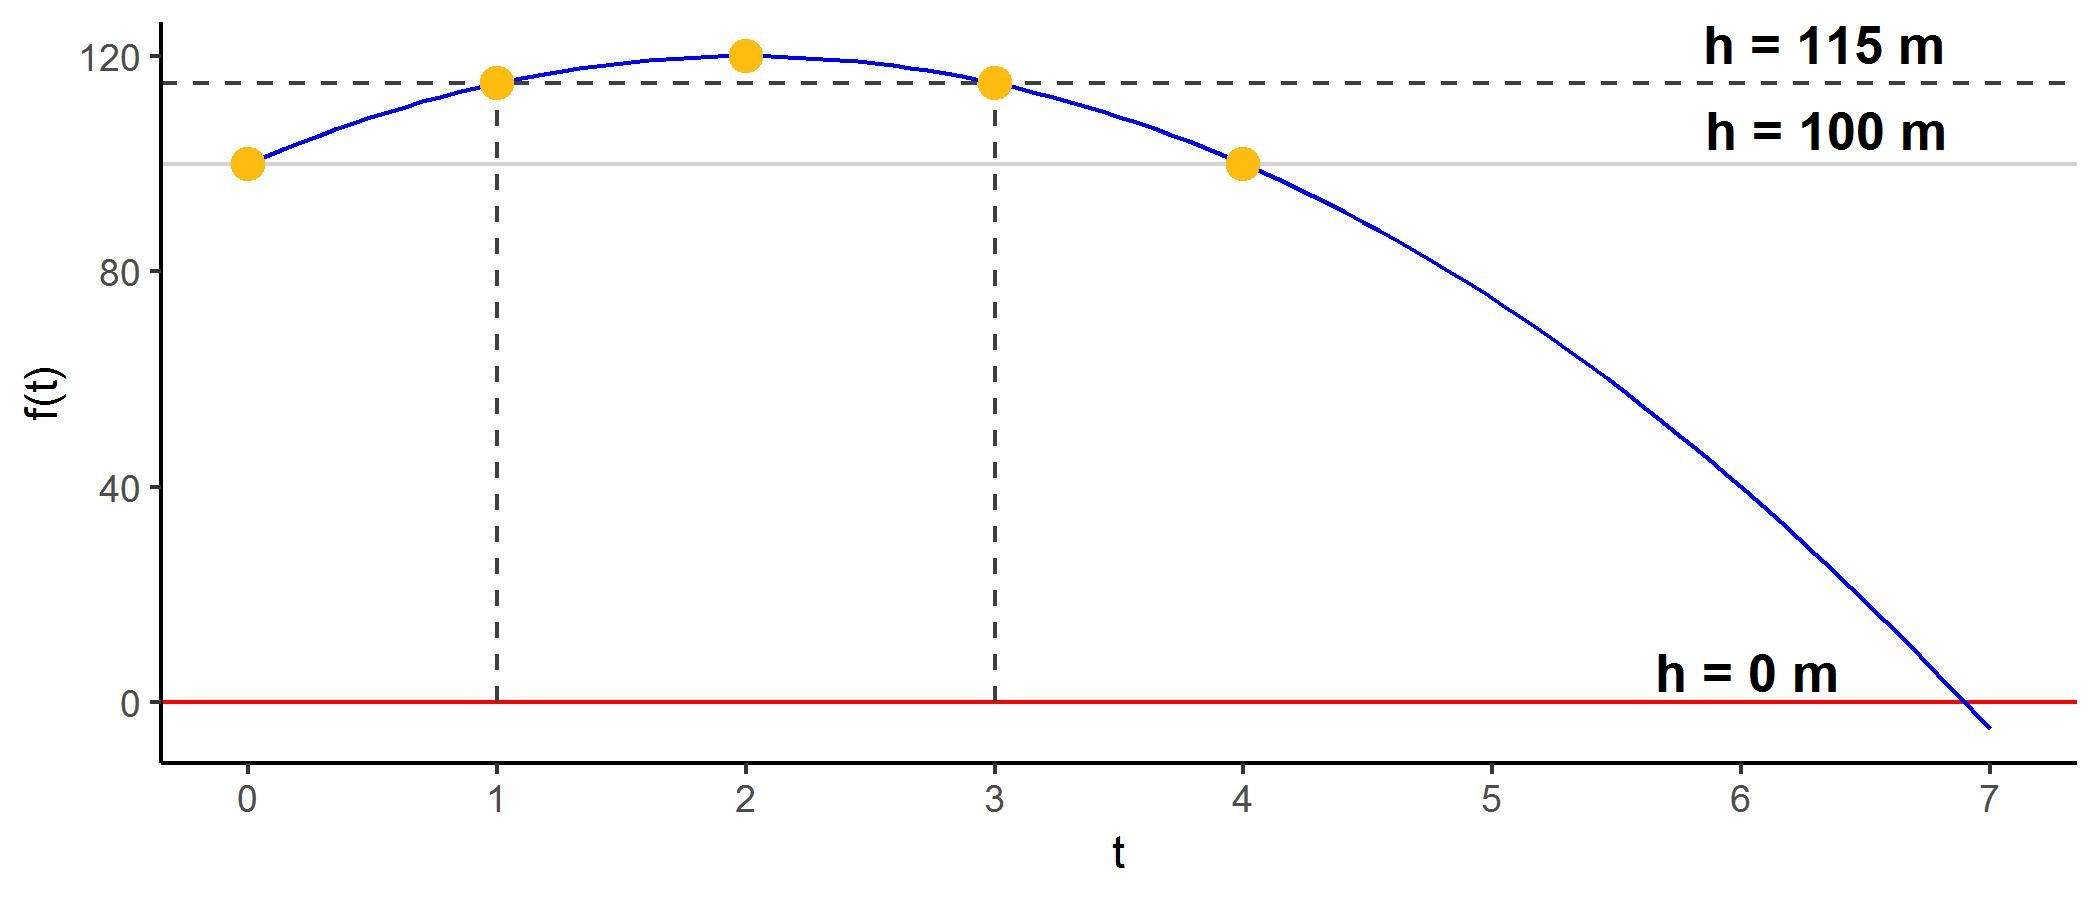
\includegraphics[scale=0.7]{img/tirar_calabaza_plot.jpg}
\end{figure}

Como vemos, justamente desde $t = 3 \, seg$ en adelante, la calabaza empieza a bajar.

Entonces, ¿por qué $f'(1)$ es positiva y $f'(3)$ es negativa cuando tanto $f(1)$ y $f(3)$ son positivas? Esto se debe a, como pudimos ver recién, que la velocidad instantánea en $t = 1$ (i.e., $f'(1)$) está ocurriendo cuando \underline{$f(t)$ está aumentando}, mientras que la velocidad instantánea que toma la calabaza en $t = 3$ ocurre cuando \underline{$f(t)$ está disminuyendo}. En otras palabras, \textbf{\underline{el signo de una derivada} nos indica \underline{la dirección} en la cual está cambiando la función}. Por lo tanto, podemos decir que:

\begin{itemize}
\item Si $f'(a) > 0$, entonces $f$ está \underline{creciendo} en $a$.
\item Si $f'(a) < 0$, entonces $f$ está \underline{decreciendo} en $a$.
\end{itemize}

Ahora calculemos cuál es la velocidad instantánea que toma la calabaza en, exactamente, $t = 2 \, seg$.
\[f'(2) = \lim_{t \to 2} \left[\frac{f(t) - f(2)}{t - 2}\right]\]
\[f'(2) = \lim_{t \to 2} \left[\frac{(100 + 20t - 5t^{2}) - 120}{t - 2}\right]\]
\[f'(2) = \lim_{t \to 2} \left[\frac{-20 + 20t - 5t^{2}}{t - 2}\right]\]
\[f'(2) = \frac{\lim_{t \to 2} [-20 + 20t - 5t^{2}]}{\lim_{t \to 2} [t - 2]}\]
\[f'(2) = \frac{-20 + 20(2) - 5(2^{2})}{2 - 2}\]
\[f'(2) = \frac{-20 + 20(2) - 5(2^{2})}{0}\]
\[f'(2) = \frac{0}{0}\]
Factoricemos el numerador de la función:
\[f'(2) = \lim_{t \to 2} \left[\frac{(100 + 20t - 5t^{2}) - 120}{t - 2}\right]\]
\[f'(2) = \lim_{t \to 2} \left[\frac{-20 + 20t - 5t^{2}}{t - 2}\right]\]
\[f'(2) = \lim_{t \to 2} \left[\frac{-5(4 - 4t + t^{2})}{t - 2}\right]\]
\[f'(2) = \lim_{t \to 2} \left[\frac{-5(t - 2)^{2}}{t - 2}\right]\]
\[f'(2) = \lim_{t \to 2} [-5(t - 2)]\]
\[f'(2) = -5(2 - 2)\]
\[f'(2) = -5(0)\]
\[f'(2) = 0\]
La velocidad instantánea en $t = 2 \, seg$, es de 0 m/s. ¿\underline{Qué significa que la derivada sea igual a cero}? Volvamos a revisar la gráfica de la página 11, pero en $t = 2 \, seg$.

\begin{figure}[hbt!]
\centering
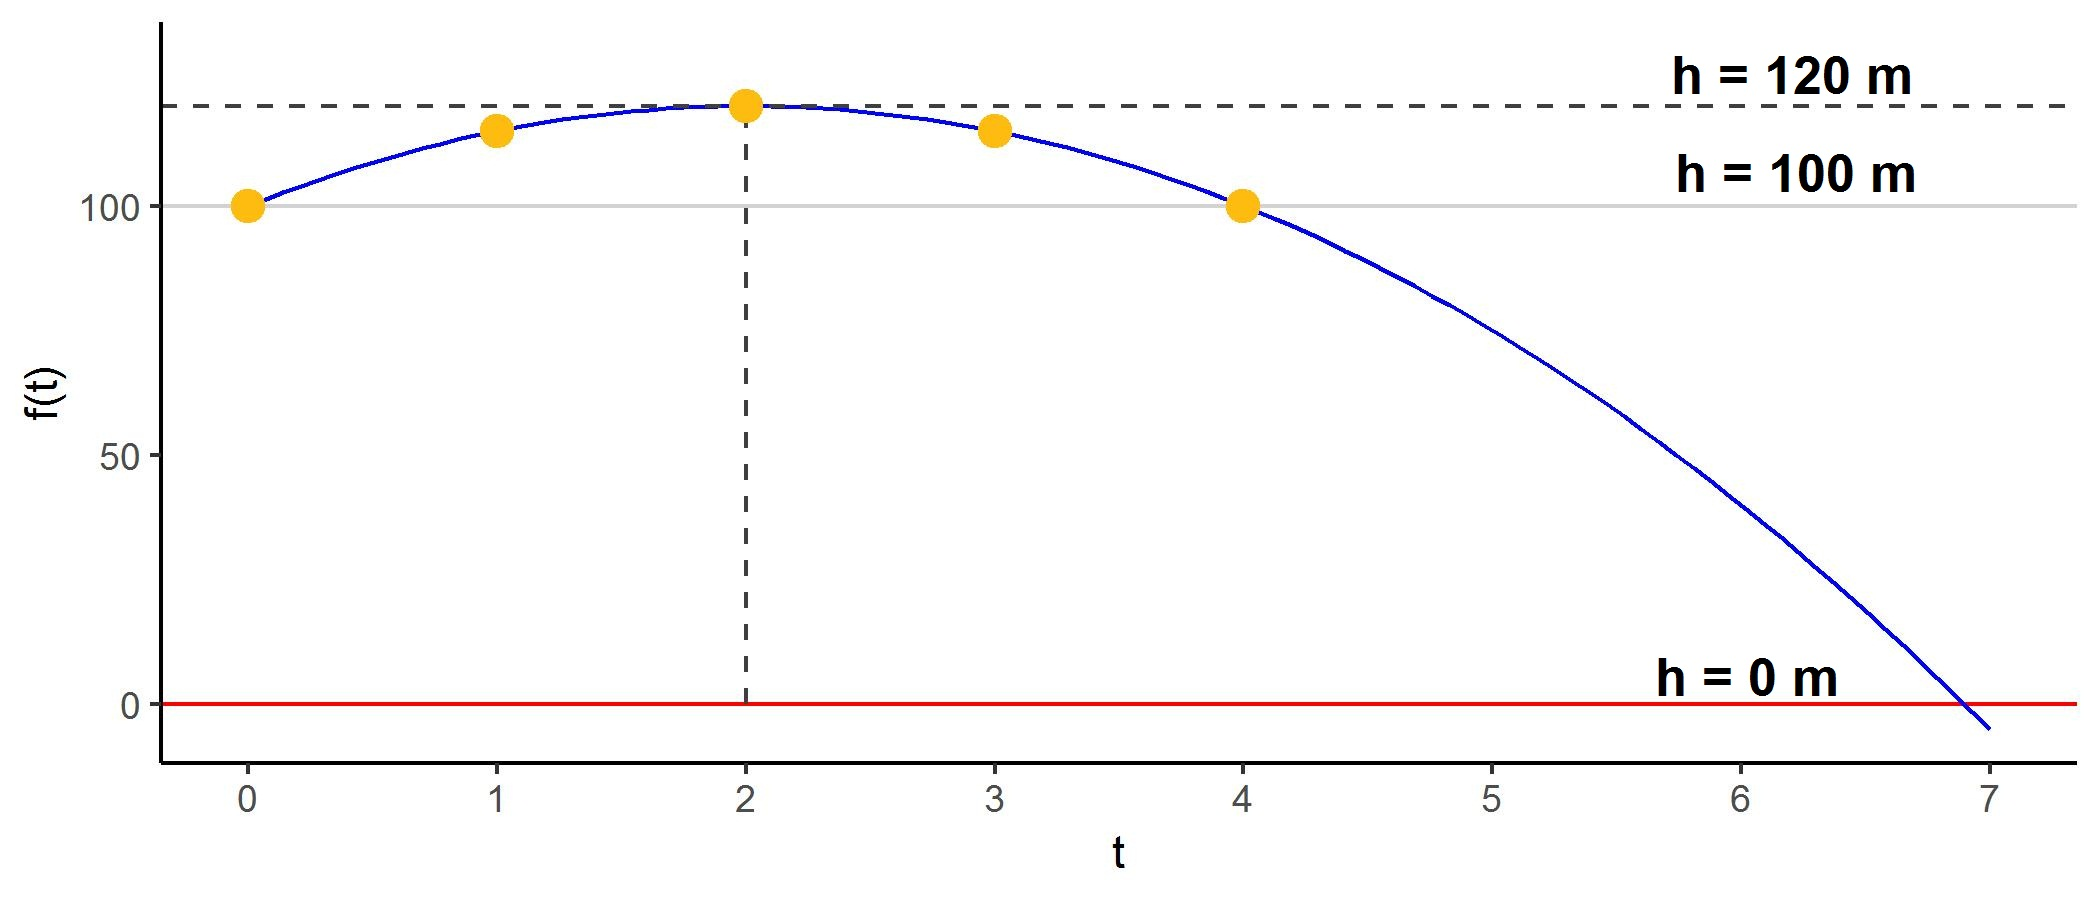
\includegraphics[scale=0.7]{img/tirar_calabaza_plot_2.jpg}
\end{figure}

Como se puede apreciar, cuando $t = 2$ la calabaza alcanza una altura ($h$) de 120 m y, al segundo siguiente ($t = 3$), ésta comienza a bajar ($f(3) = 115 \, m$). En otras palabras, en aquel punto la calabaza alcanza su altura máxima, por lo tanto, su velocidad instantánea exactamente en $t = 2$ va a ser cero, puesto que de ahí en adelante comenzará a bajar y, como vimos anteriormente, desde $t = 3$ en adelante, la velocidad instantánea empieza a ser negativa.

Por consiguiente, podemos interpretar que \textbf{cuando la derivada de una función es igual a cero (i.e., $f'(x) = 0$), quiere decir que dicha función alcanzó su punto máximo} por lo que, en puntos posteriores, $f$ decrecerá y $f'$, por tanto, será negativa.



\subsection{Líneas Tangentes.}

En esta ocasión analizaremos a la derivada desde un punto de vista geométrico. En las secciones anteriores, la analizamos desde una perspectiva física y ahora nos concentraremos en el siguiente problema geométrico.

Digamos que tenemos una función $y = f(x)$ (línea celeste) y lo que queremos saber es cuál es la línea tangente (línea naranja) que, de algún modo, sabemos dibujar intuitivamente, como lo podemos ver en la siguiente imagen.

\begin{figure}[hbt!]
\centering
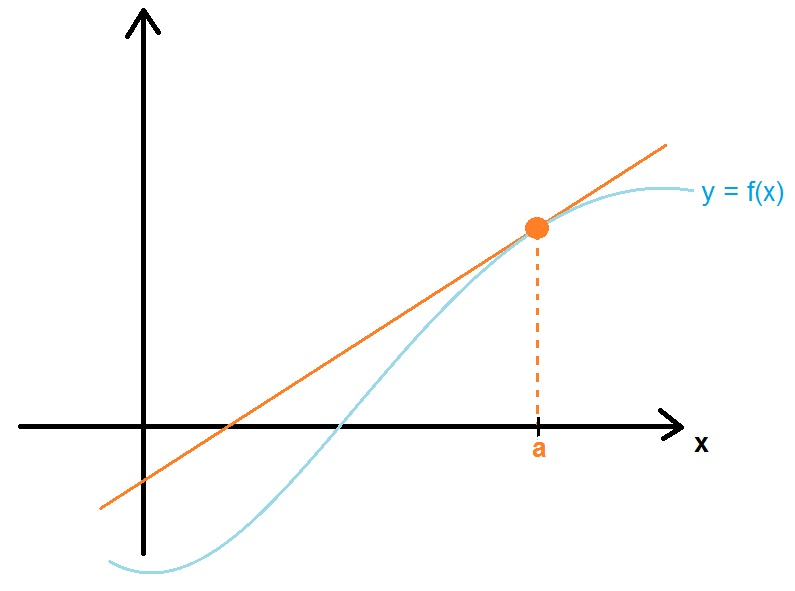
\includegraphics[scale=0.5]{img/tangent_line_intro.jpg}
\end{figure}

\newpage

Ahora bien, si queremos entender mejor a la línea tangente, debemos recordar que ésta es una ``\underline{línea}'', por lo tanto, para comprenderla es suficiente con conocer \underline{un punto} de ella y su \underline{pendiente}:

\begin{itemize}
\item Punto $(x_{0}, \, y_{0})$
\item pendiente $m$.
\end{itemize}

Como podemos observar, el gráfico de arriba ya nos entrega la primera información, puesto que $x = a$ e $y = f(a)$. Es decir:

\begin{itemize}
\item Punto $(x_{0}, \, y_{0}) = (a, \, f(a))$
\end{itemize}

Por otra parte, para calcular la línea tangente podemos usar la ecuación de la recta punto-pendiente:
\[y - y_{0} = m(x - x_{0})\]
Conocemos los valores de $x_{0} = a$ y de $y_{0} = f(a)$, por lo tanto:
\[y - f(a) = m(x - a)\]
Ahora tenemos un problema realmente simple, lo que queremos buscar es la pendiente $m$ de la linea tangente y es aquí en donde entra el Cálculo como tal.

En las siguientes secciones aprenderemos que \underline{$m = f'(a)$}. En otras palabras, \textbf{la pendiente de la línea tangente corresponde a la derivada de la función en donde se busca dicha línea tangente} (como en la imagen de arriba).

\newpage

1.5.a) \underline{Intuición de la Línea Tangente}.

Comúnmente se suele definir o entender que una línea tangente es aquella que, al trazarla sobre una curva, la toca en un punto sobre ella. El problema de este punto de vista es que solo se aplica si la curva es un círculo, pero en muchas otras funciones no ocurre así. En esto iremos profundizando más adelante, pero por ahora acerquémonos a esta línea de forma intuitiva.

Veamos a continuación la gráfica de la función $f(x) = 0.5x^{3}-x$, en la cual se encuentra marcado, por medio de un círculo naranjo, el punto $(-1, \, 0.5)$.

En la gráfica podemos observar dos curvas pronunciadas en ella. Ahora, haremos una especie de ``zoom'' justo donde está el punto $(-1, \, 0.5)$. Mantendremos todo igual y nos acercaremos al rango de valores que va desde $x \approx -1.02$ y $x \approx -0.98$.

Como es posible apreciar, a medida que nos acercamos a la curva de la función $f(x) = 0.5x^{3}-x$ en un punto determinado de ella, que en este caso fue en $x = -1$, visualmente va haciéndose más recta y, precisamente, \textbf{la línea recta que se forma corresponde a nuestra \underline{línea tangente}}. Esto quiere decir que dicha línea debe apuntar en la misma dirección en que lo hace la curva de nuestra función en un punto determinado o, en otras palabras, \textbf{en cierto punto $x = a$ la pendiente de la línea tangente debe ser igual a la pendiente de nuestra función en aquel punto}.



\subsection{Línea Secante.}

Anteriormente dijimos que queremos calcular la pendiente de una recta tangente. Para ésto, introduciremos un nuevo concepto: la línea secante. Con el fin de entenderla, la dibujaremos a continuación:

\newpage

\begin{figure}[hbt!]
\centering
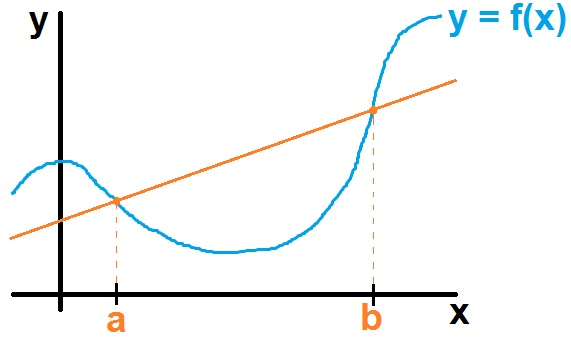
\includegraphics[scale=0.7]{img/secant_line_intro.jpg}
\end{figure}

Como podemos observar, la \textbf{línea secante} de la recta curva $y = f(x)$ es aquella que \textbf{la toca en 2 puntos a lo largo de ella}.

Ahora bien, si nos preguntamos cuál es la pendiente de esta recta secante, podemos observar que tenemos dos puntos definidos en ella: $(a, f(a))$ y $(b, f(b))$ y lo que podemos hacer es ver la distancia que hay entre ellas. Es decir, el \underline{cambio} (i.e., $\Delta$) que hay entre $x = a$ y $x = b$, así como entre $y = f(a)$ y $y = f(b)$, lo cual geométricamente se ve de esta manera:

\begin{figure}[hbt!]
\centering
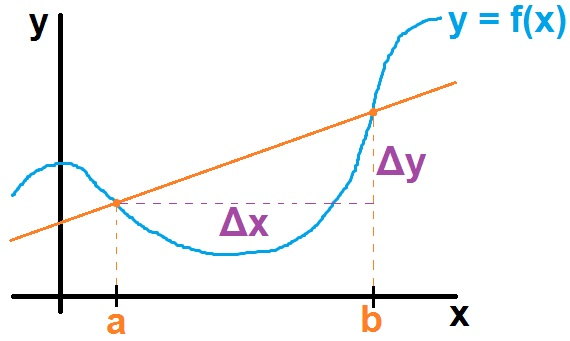
\includegraphics[scale=0.7]{img/secant_line_intro_2.jpg}
\end{figure}

\newpage

Dichos cambios nos permiten obtener la \underline{pendiente de la línea secante}, la que calculamos como:
\[m = \frac{\Delta y}{\Delta x}\]
En ese sentido, $\Delta y = \Delta f$, de manera que $\Delta f = f(b)-f(a)$. Mientras que $\Delta x = b - a$, por consiguiente si reemplazamos la fórmula de arriba con la información que acabamos de observar, la pendiente de la recta secante será:
\[m = \frac{\Delta y}{\Delta x}\]
\[m = \frac{\Delta f}{\Delta x}\]
\[m = \frac{f(b)-f(a)}{b-a}\]
Así es, la fórmula de la \textbf{pendiente de la secante} corresponde a la \textbf{tasa de cambio promedio de $f(x)$ con respecto a $x$}. En otras palabras, \textbf{dicha pendiente es la que mide la tasa de cambio promedio}.

Ahora bien, ¿cómo se vincula la pendiente de la línea secante con la de la línea tangente? Lo hace a partir de la aproximación de un punto hacia otro. En otras palabras, a medida que el punto $x = b$ se \underline{acerca} al punto $x = a$, \textbf{la pendiente de la recta secante pasa a acercarse a la pendiente de la recta tangente}, lo cuál como vimos antes, lo podemos expresar matemáticamente de la siguiente manera:
\[m_{t} = \lim_{b \to a} m_{s}\]
\[m_{t} = \lim_{b \to a} \frac{f(b)-f(a)}{b-a}\]
Por consiguiente, a partir de lo que mencionamos anteriormente (pág. 6-7), también podemos decir que \textbf{la pendiente de la recta tangente corresponde a la derivada de una función en un punto}:
\[m = f'(a)\]
De este modo, a partir de lo que hemos aprendido hasta ahora en todas estas páginas, tenemos \underline{tres interpretaciones} de lo que es una derivada en un punto: una geométrica, otra simbólica y una física.

Por lo tanto, a medida que $b \to a$:

\begin{enumerate}
\item \underline{Geométrica}: 

\centerline{Pendiente línea secante $\to$ Pendiente línea tangente}

\item \underline{Simbólica}:
\[\frac{f(b)-f(a)}{b-a} \to f'(a)\]

\item \underline{Física}: 

\centerline{Tasa de cambio promedio $\to$ Tasa de cambio instantánea}

\end{enumerate}

A partir de esto último también podemos señalar que la derivada de una función en un punto o \underline{$f'(a)$} es tanto una \underline{tasa de cambio instantánea} como la \underline{pendiente de una línea tangente}.



\subsection{La Existencia de las Líneas Tangentes y de las Derivadas.}

Hay algunos casos de funciones en donde no existe una línea tangente, de manera que no existe una derivada en ella.

Veamos, por ejemplo, la \underline{función valor absoluto} o $f(x) = |x|$

\newpage

\begin{figure}[hbt!]
\centering
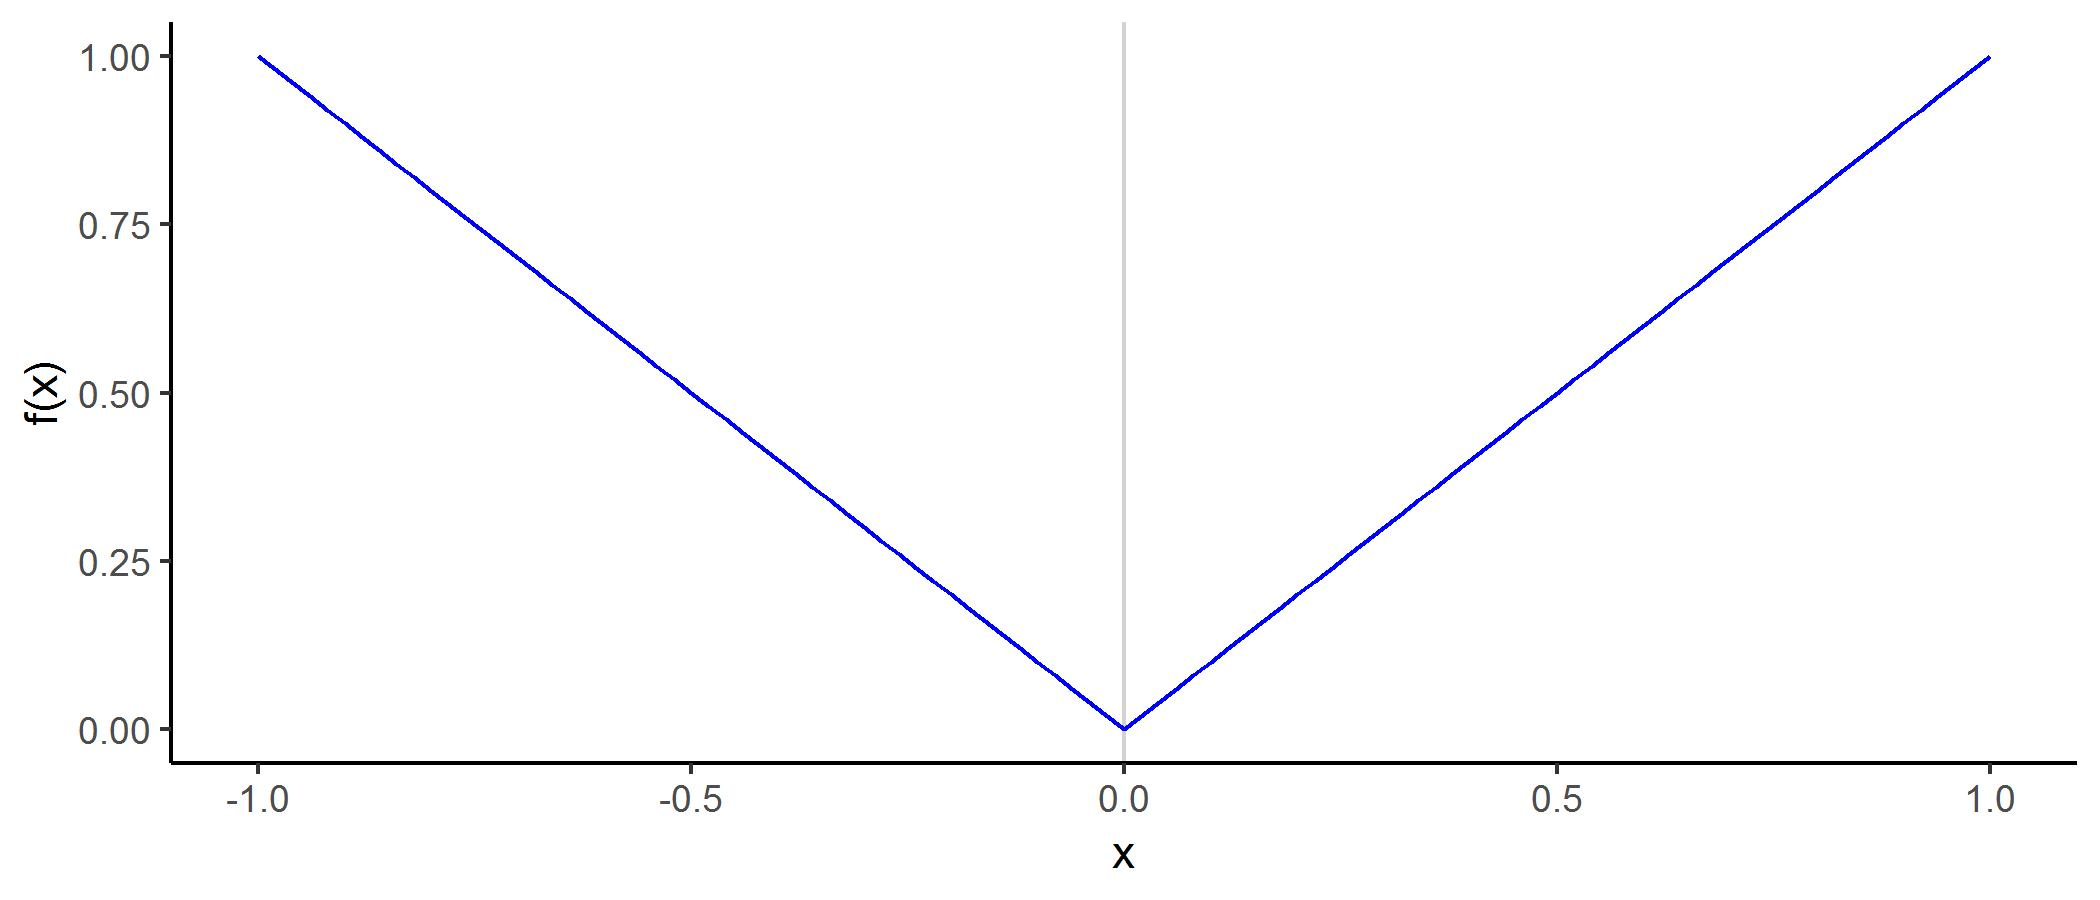
\includegraphics[scale=0.7]{img/abs_fun_plot.jpg}
\end{figure}

Como se puede observar en el origen o el punto (0, 0) de la función, hay una \underline{esquina}.

Otro ejemplo es la \underline{función Heaviside} (más info sobre ella, por \href{https://es.wikipedia.org/wiki/Funci%C3%B3n_escal%C3%B3n_de_Heaviside}{acá}.) la cuál, como podremos apreciar, tiene un \underline{salto de discontinuidad} (\textit{jump discontinuity}) en $x = 0$.

\begin{figure}[hbt!]
\centering
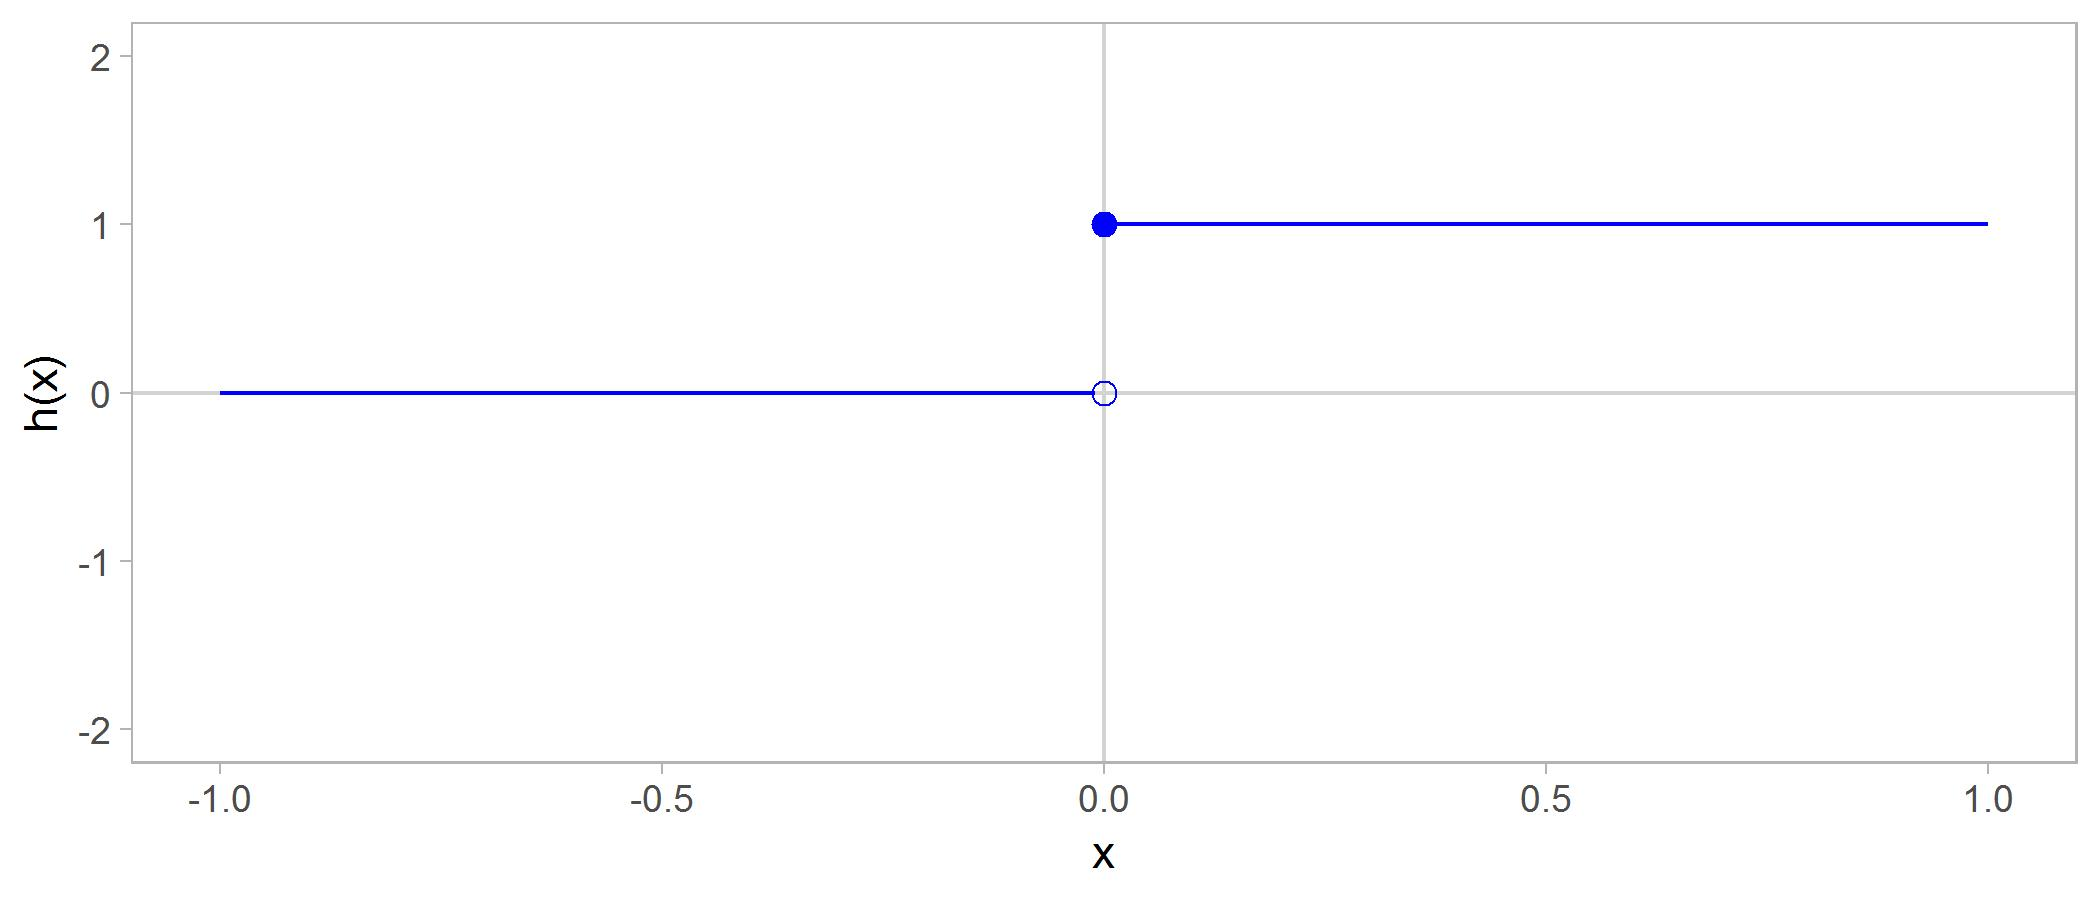
\includegraphics[scale=0.7]{img/heaviside_plot.jpg}
\end{figure}

Veamos ambas funciones en mayor detalle.

\newpage

a) \underline{Función Valor Absoluto}.

Como se puede observar en la gráfica de la función valor absoluto de arriba, en $x = 0$ no existe una línea tangente\footnote{Si, intuitivamente, hicieramos zoom en aquel punto, no podríamos ver una línea que se forma en dicho punto.}. Sin embargo, digamos que cubrimos con una mano la parte izquierda de la gráfica, desde $x = 0$ hacia atrás.

\begin{figure}[hbt!]
\centering
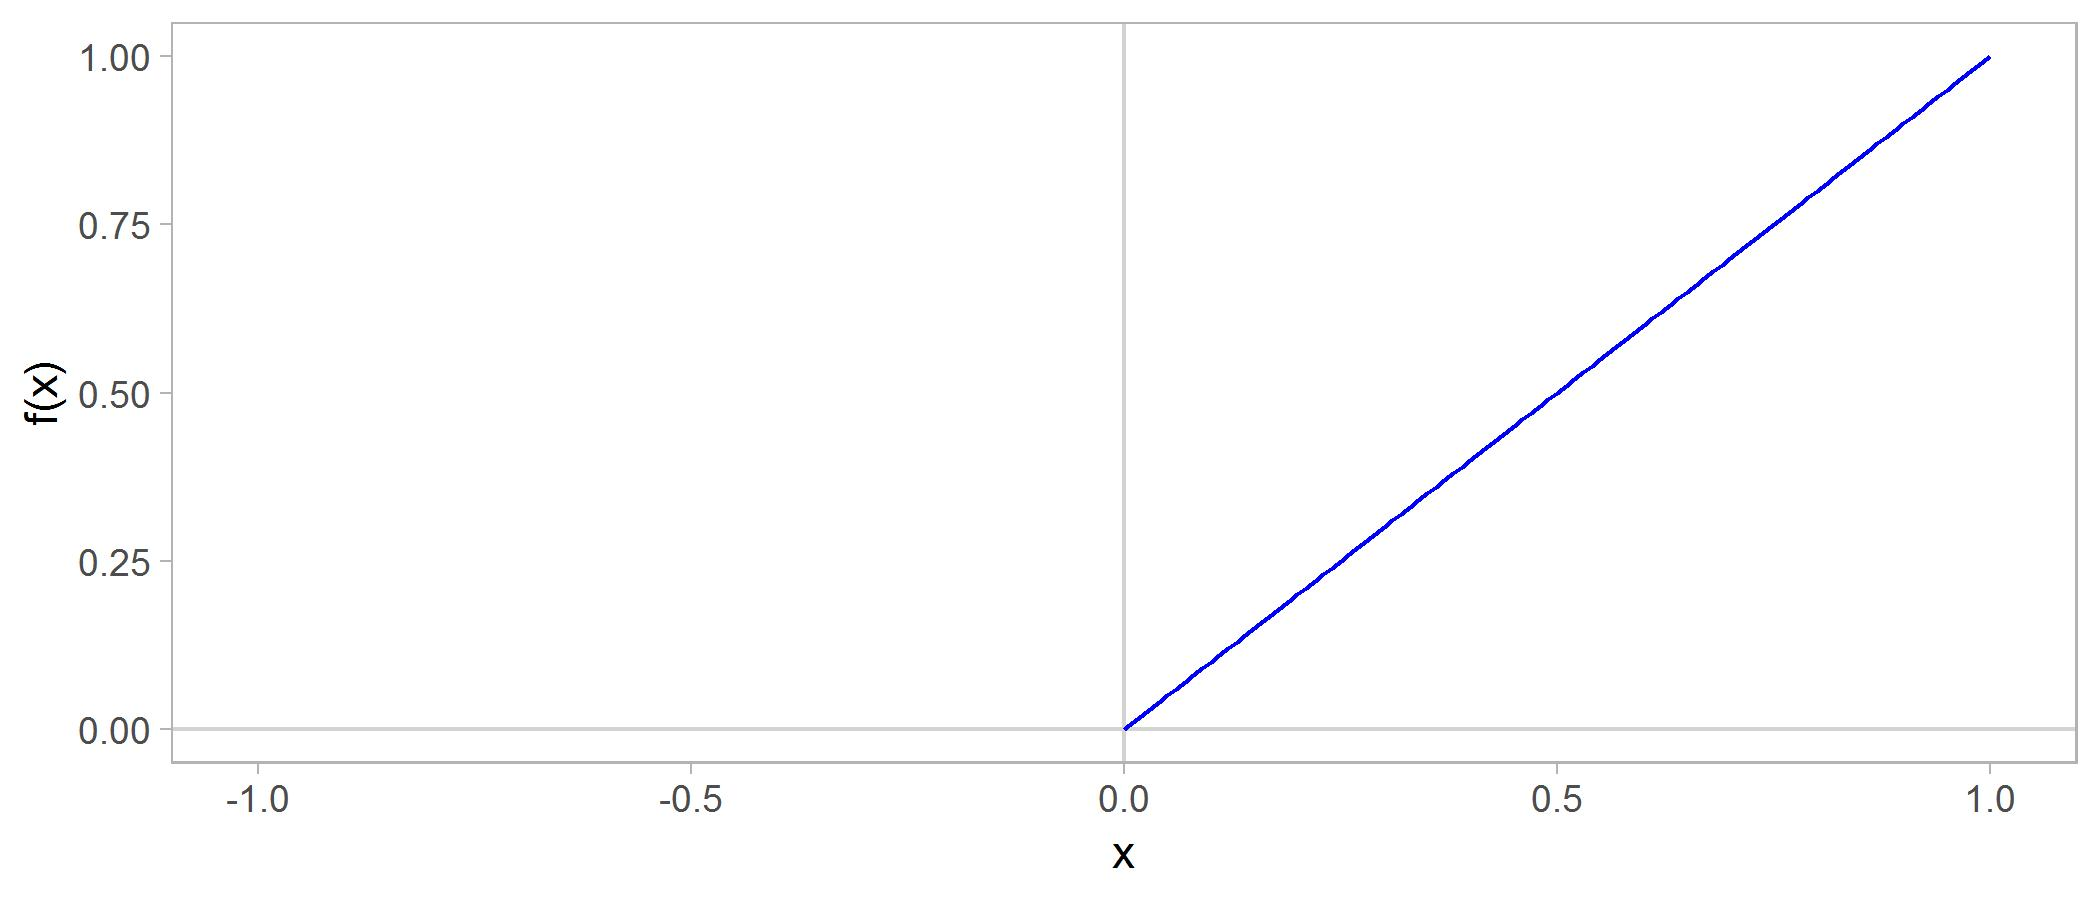
\includegraphics[scale=0.7]{img/abs_fun_right_plot.jpg}
\end{figure}

Es posible ver que, a medida que $x \to 0^{+}$, la pendiente de las líneas secantes se van acercando a la pendiente del gráfico de arriba, la cual es $m = 1$. Por ejemplo, tomemos dos valores $x_{1} = 1$ y $x_{2} = 2$, para calcular la pendiente $m$ de $f(x) = |x|$.
\[m = \frac{f(2)-f(1)}{2-1}\]
\[m = \frac{|2|-|1|}{2-1}\]
\[m = 1\]
A lo que nos estamos refiriendo es que el \textbf{límite de la derecha} de la pendiente de las secantes de $f(x) = |x|$, a medida que $x \to 0^{+}$, va a corresponder a la \textbf{tangente} de dicha función, la cual se la denomina como la \textbf{\underline{derivada de la derecha}} y, para este caso, se la denota como $f'(0^{+})$:
\[f'(0^{+}) = \lim_{x \to 0^{+}} \frac{f(x)-f(0)}{x-0}\]
En ese sentido, como la derivada de la derecha de $f(x) = |x|$ en $x = 0^{+}$, se acerca a la $m$ de dicha función, entonces esta derivada será igual a 1:
\[f'(0^{+}) = \lim_{x \to 0^{+}} \frac{f(x)-f(0)}{x-0}\]
\[f'(0^{+}) = \lim_{x \to 0^{+}} \frac{|x|-0}{x-0}\]
\[f'(0^{+}) = 1\]
Ahora veamos qué ocurre cuando tapamos la parte derecha del gráfico.

\begin{figure}[hbt!]
\centering
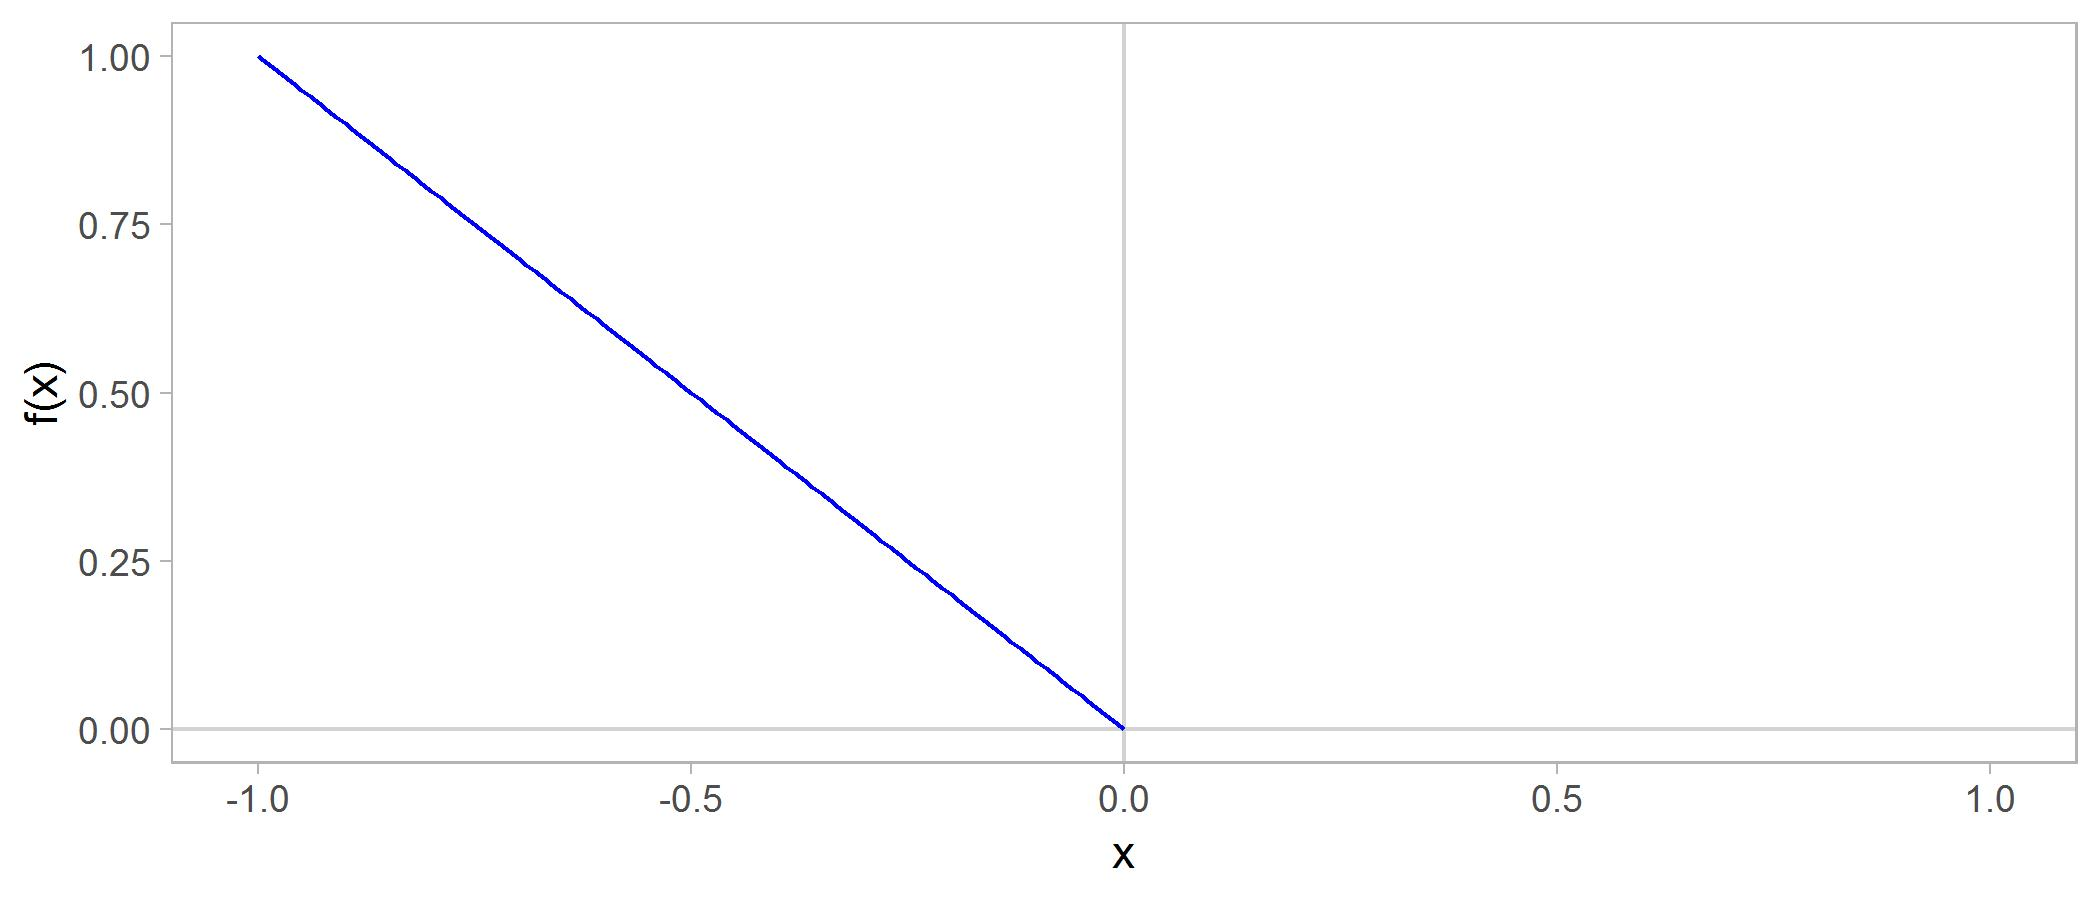
\includegraphics[scale=0.7]{img/abs_fun_left_plot.jpg}
\end{figure}

Como podemos apreciar, el gráfico de arriba tiene un límite de las líneas secantes que se va acercando desde la izquierda. En otras palabras, la pendiente de las líneas secantes de dicho gráfico se van acercando a la pendiente del mismo gráfico a medida que $x \to 0^{-}$. Lo cual nos da un \textbf{límite de la izquierda} que corresponde a la \textbf{\underline{derivada de la izquierda}}, que en este caso denotamos como $f'(0^{-})$.
\[f'(0^{-}) = \lim_{x \to 0^{-}} \frac{f(x)-f(0)}{x-0}\]
Tal como mencionamos, a medida que las líneas secantes se acercan a $x = 0$ desde la izquierda en este gráfico, las pendientes de éstas se acercan a la pendiente del gráfico y, si la calculamos, $m = -1$. Por ejemplo, tomemos dos puntos $x_{1} = -1$ y $x_{2} = -2$, entonces:
\[m = \frac{f(-2)-f(-1)}{(-2) - (-1)}\]
\[m = \frac{2-1}{-2 + 1}\]
\[m = -1\]
Por consiguiente, la derivada a la izquierda de $f(x) = |x|$, será:
\[f'(0^{-}) = \lim_{x \to 0^{-}} \frac{f(x)-f(0)}{x-0}\]
\[f'(0^{-}) = \lim_{x \to 0^{-}} \frac{|x|-f(0)}{x-0}\]
\[f'(0^{-}) = -1\]
Ahora bien, como pudimos ver, tanto la derivada de la izquierda como de la derecha, existen. Sin embargo, no son iguales:
\[f'(0^{+}) \neq f'(0^{-})\]
Por lo tanto, podemos señalar que la derivada de la función $f(x) = |x|$, \underline{no existe} en $x = 0$.


b) \underline{Función Heaviside}.

En la gráfica de la función Heaviside (pág. 20) pudimos observar que en $x = 0$ hay un salto de discontinuidad, el cual está denotado con un círculo vacío.

Si hacemos lo mismo que en la función valor absoluto, lo de cubrir con una mano la parte izquierda del gráfico, podemos ver que en $x = 0$ la función Heaviside es igual a $1$ ($h(0) = 1$) y tiene una \underline{derivada de la derecha} $h'(0^{+})$.

\newpage

\begin{figure}[hbt!]
\centering
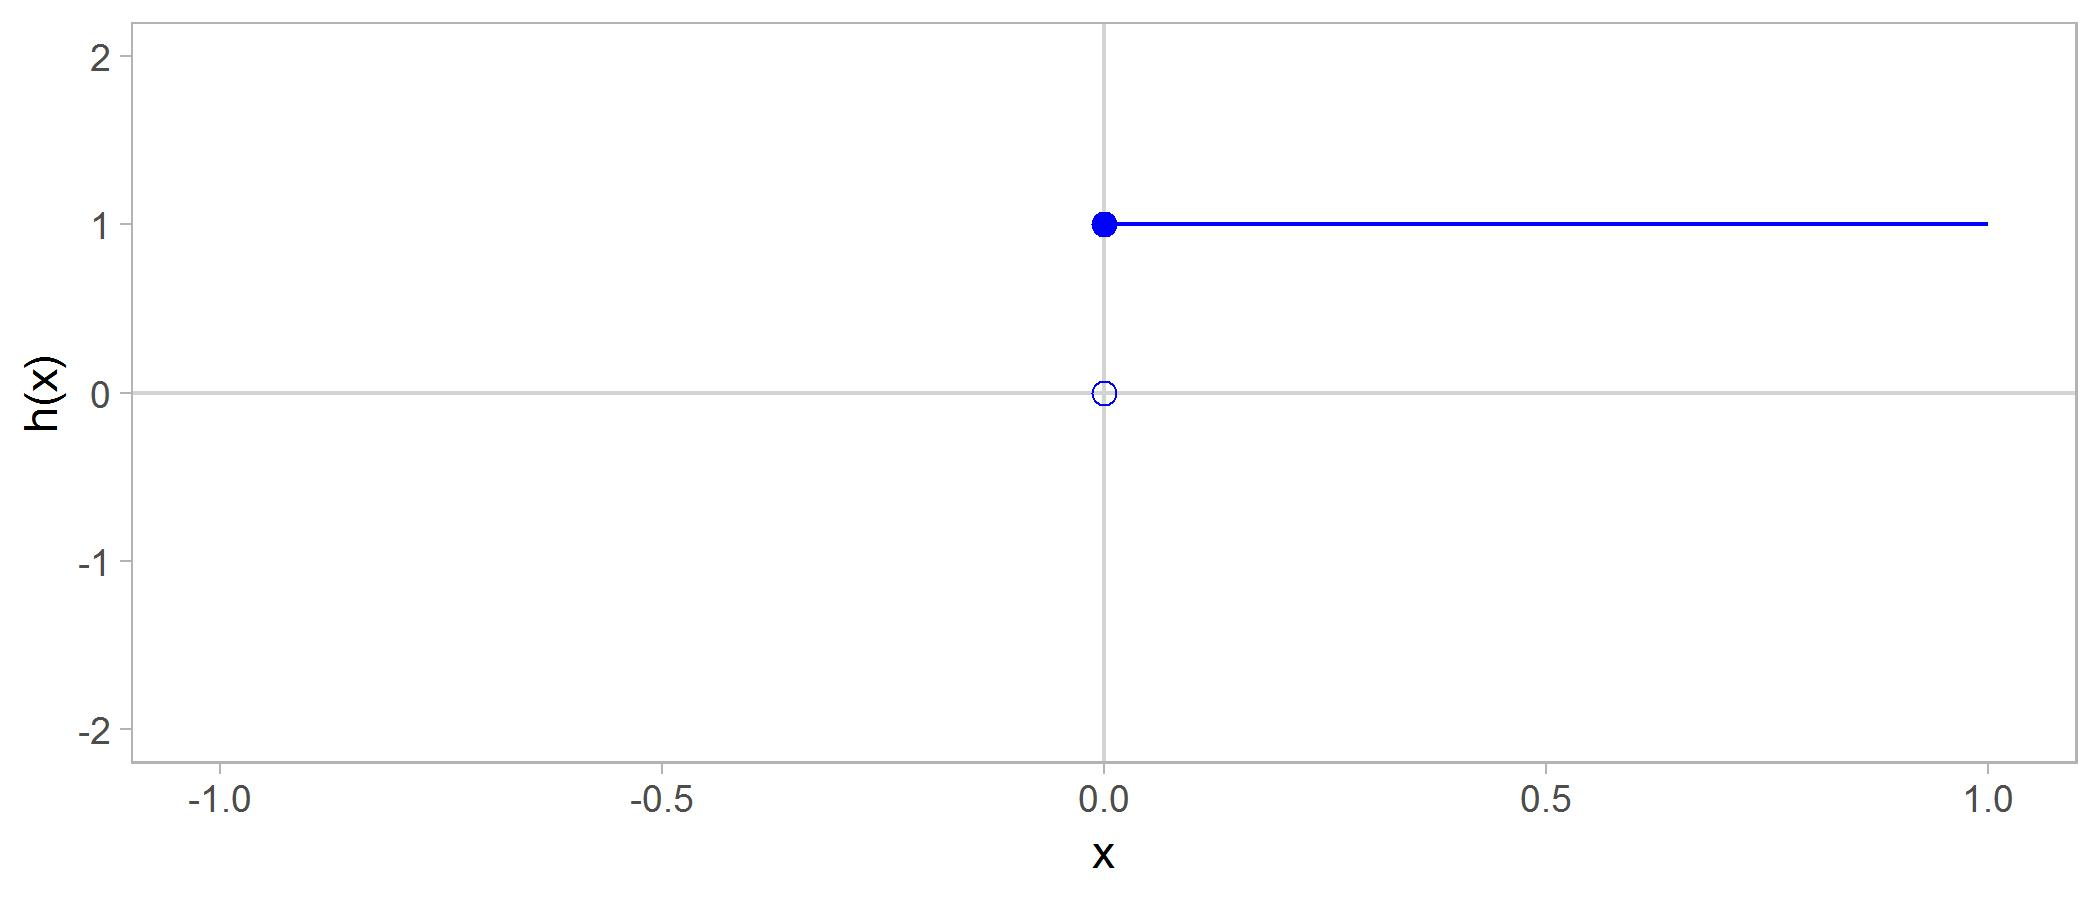
\includegraphics[scale=0.7]{img/heaviside_right_plot.jpg}
\end{figure}

En este caso, cuando $x = 0^{+}$, la pendiente de $h(x)$ es $m = 0$ (i.e., no tiene pendiente) y, como la pendientes de las secantes se acercan a dicha pendiente a medida que $x \to 0^{+}$, entonces la derivada a la derecha de la misma función también será igual a cero:
\[h'(0^{+}) = \lim_{x \to 0^{+}} \frac{h(x)-h(0)}{x-0}\]
\[h'(0^{+}) = 0\]
Por otra parte, si cubrimos el lado derecho de la gráfica de la función Heaviside, podemos ver que en todos los valores de $x$ que están a la izquierda de cero, $h(x) = 0$ salvo en $x = 0$, en donde esta función salta para ser igual a $1$.

\begin{figure}[hbt!]
\centering
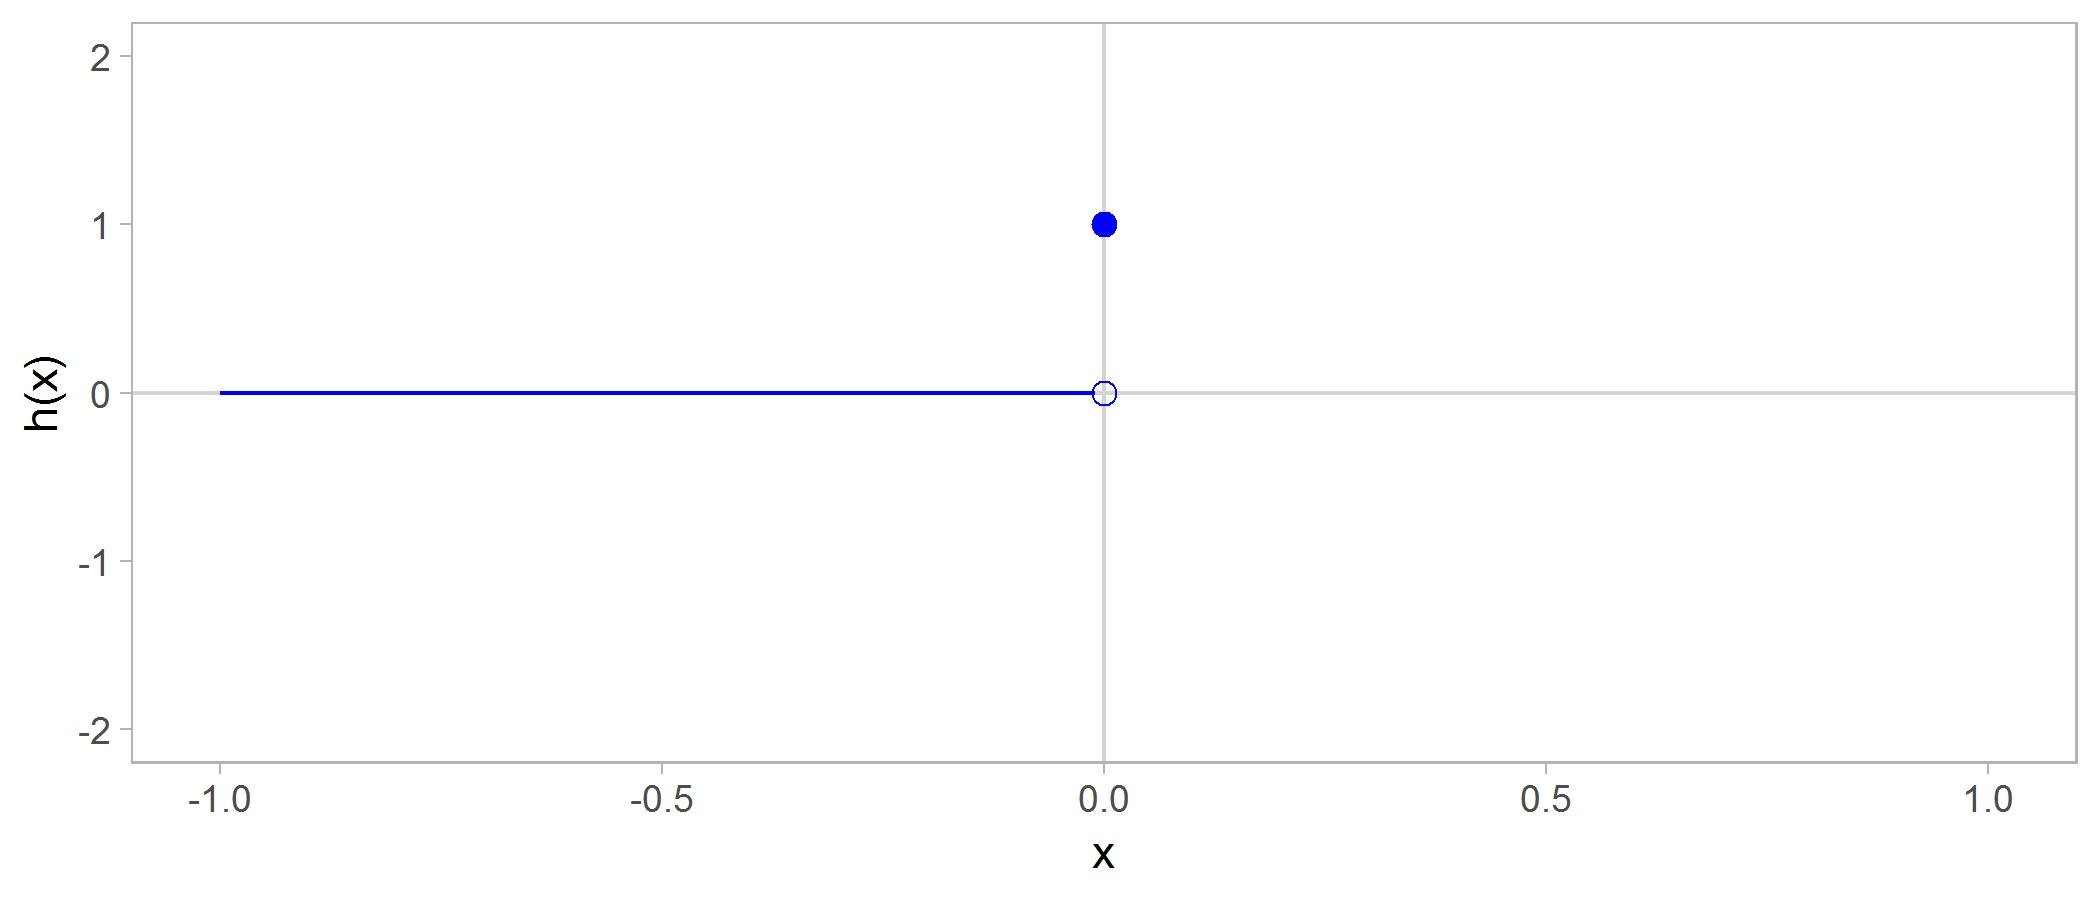
\includegraphics[scale=0.7]{img/heaviside_left_plot.jpg}
\end{figure}

Acá, a medida que $x \to 0^{-}$, la pendiente de las líneas secantes se van acercando a la \underline{línea vertical} que se forma entre $x = 0$ y $h(x) = 0$. En otras palabras, la \underline{derivada de la izquierda} de la función Heaviside en $x = 0$ será igual al infinito.
\[h'(0^{-}) = \lim_{x \to 0^{-}} \frac{h(x)-h(0)}{x-0}\]
\[h'(0^{-}) = \infty\]
Por consiguiente, otra vez las derivadas a la izquierda y a la derecha en $x = 0$ de la función Heaviside $h(x)$, existen, pero no son iguales, lo cual significa que \underline{la derivada en el punto $x = 0$} de esta función, \underline{no existe}.
\[h'(0^{+}) \neq h'(0^{-})\]
En los casos de las dos funciones que acabamos de ver, observamos la situación en donde en un punto no existe la derivada puesto que no existe una línea tangente allí. Es decir:

\centerline{No existe línea tangente $\Rightarrow$ No existe derivada}

Pero \textbf{si existe la línea tangente en un punto de una función, ¿entonces también existirá su derivada en dicho punto?} La respuesta es \textbf{\underline{sí}, aunque \underline{excepto} para el caso de las \underline{líneas tangentes verticales}}.

Por ejemplo, veamos el caso de la función raíz cúbica $g(x) = \sqrt[3]{x}$.

\begin{figure}[hbt!]
\centering
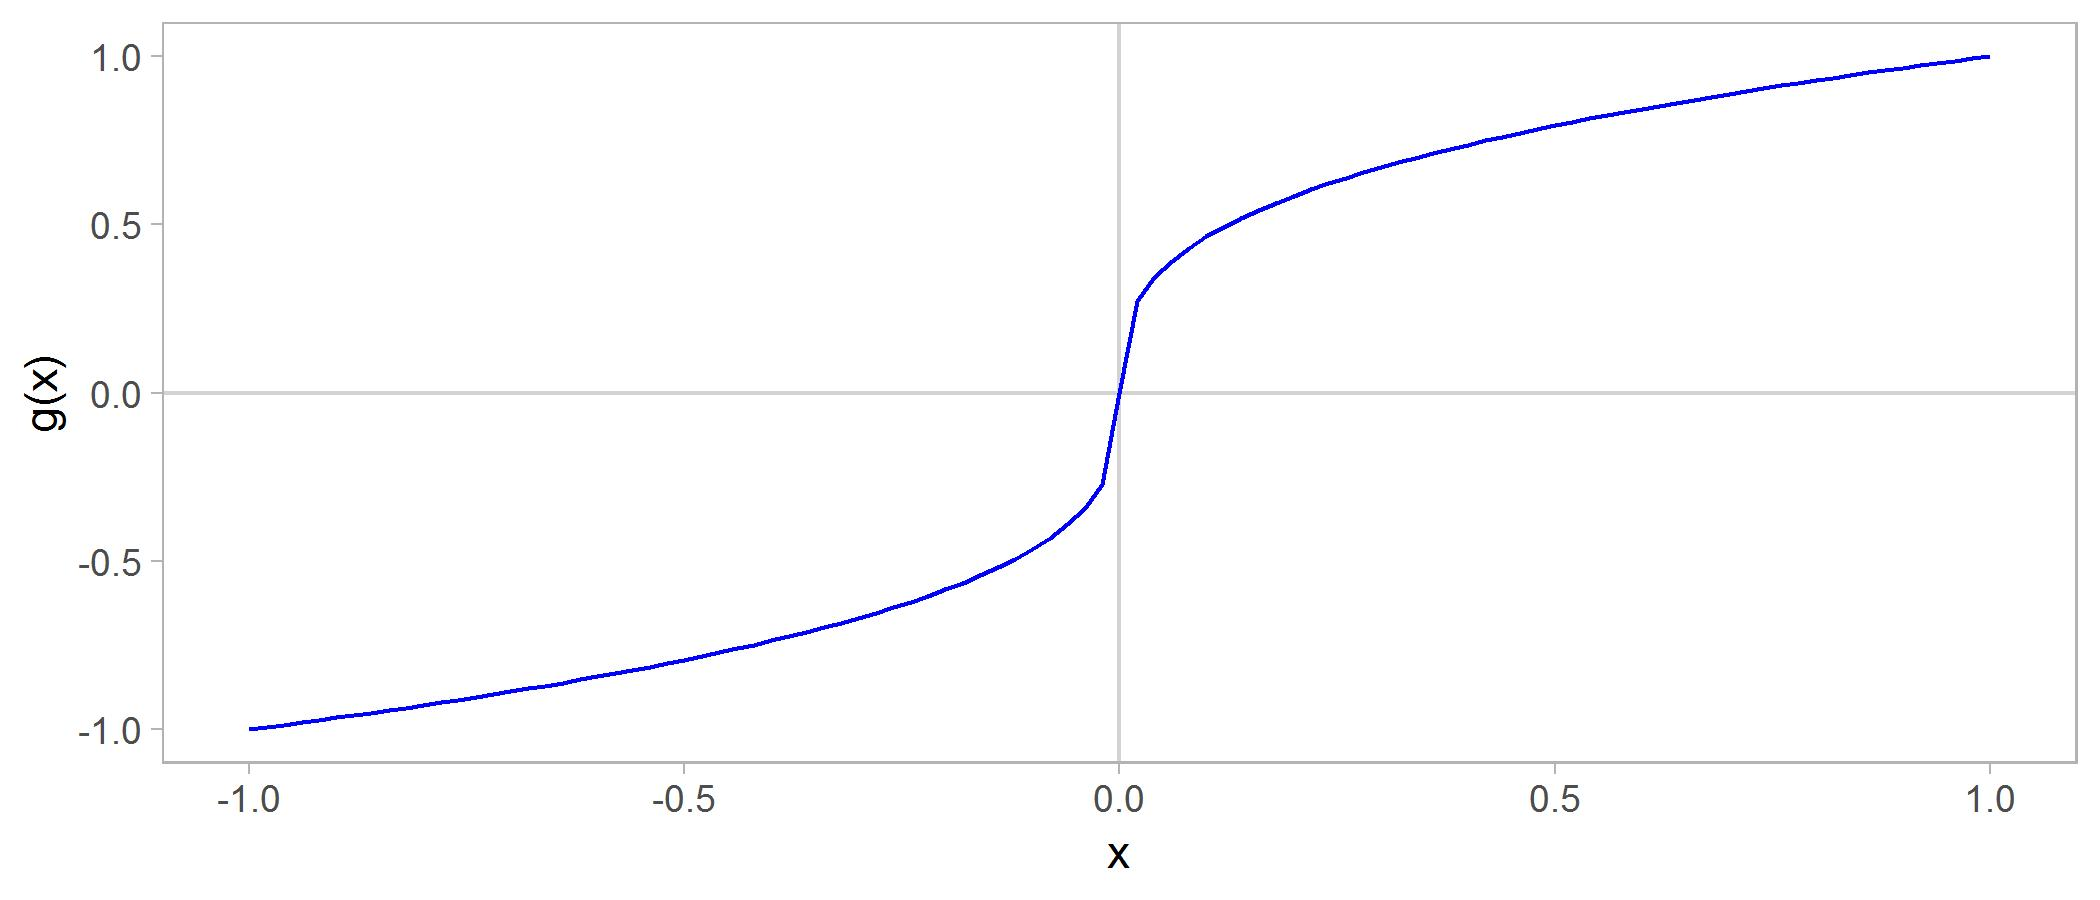
\includegraphics[scale=0.7]{img/cubic_root_plot.jpg}
\end{figure}

En este caso, la tangente en $x = 0$ está definida para la función $g(x) = \sqrt[3]{x}$, sin embargo, en dicho punto va a ser una línea vertical, por consiguiente, \underline{existe la línea tangente}, \underline{pero no la derivada} en $x = 0$.


\subsection{La Derivada de la Segunda Potencia.}

En esta ocasión, nos concentraremos en la función $f(x)= x^{2}$, cuya gráfica es la siguiente parábola.

\begin{figure}[hbt!]
\centering
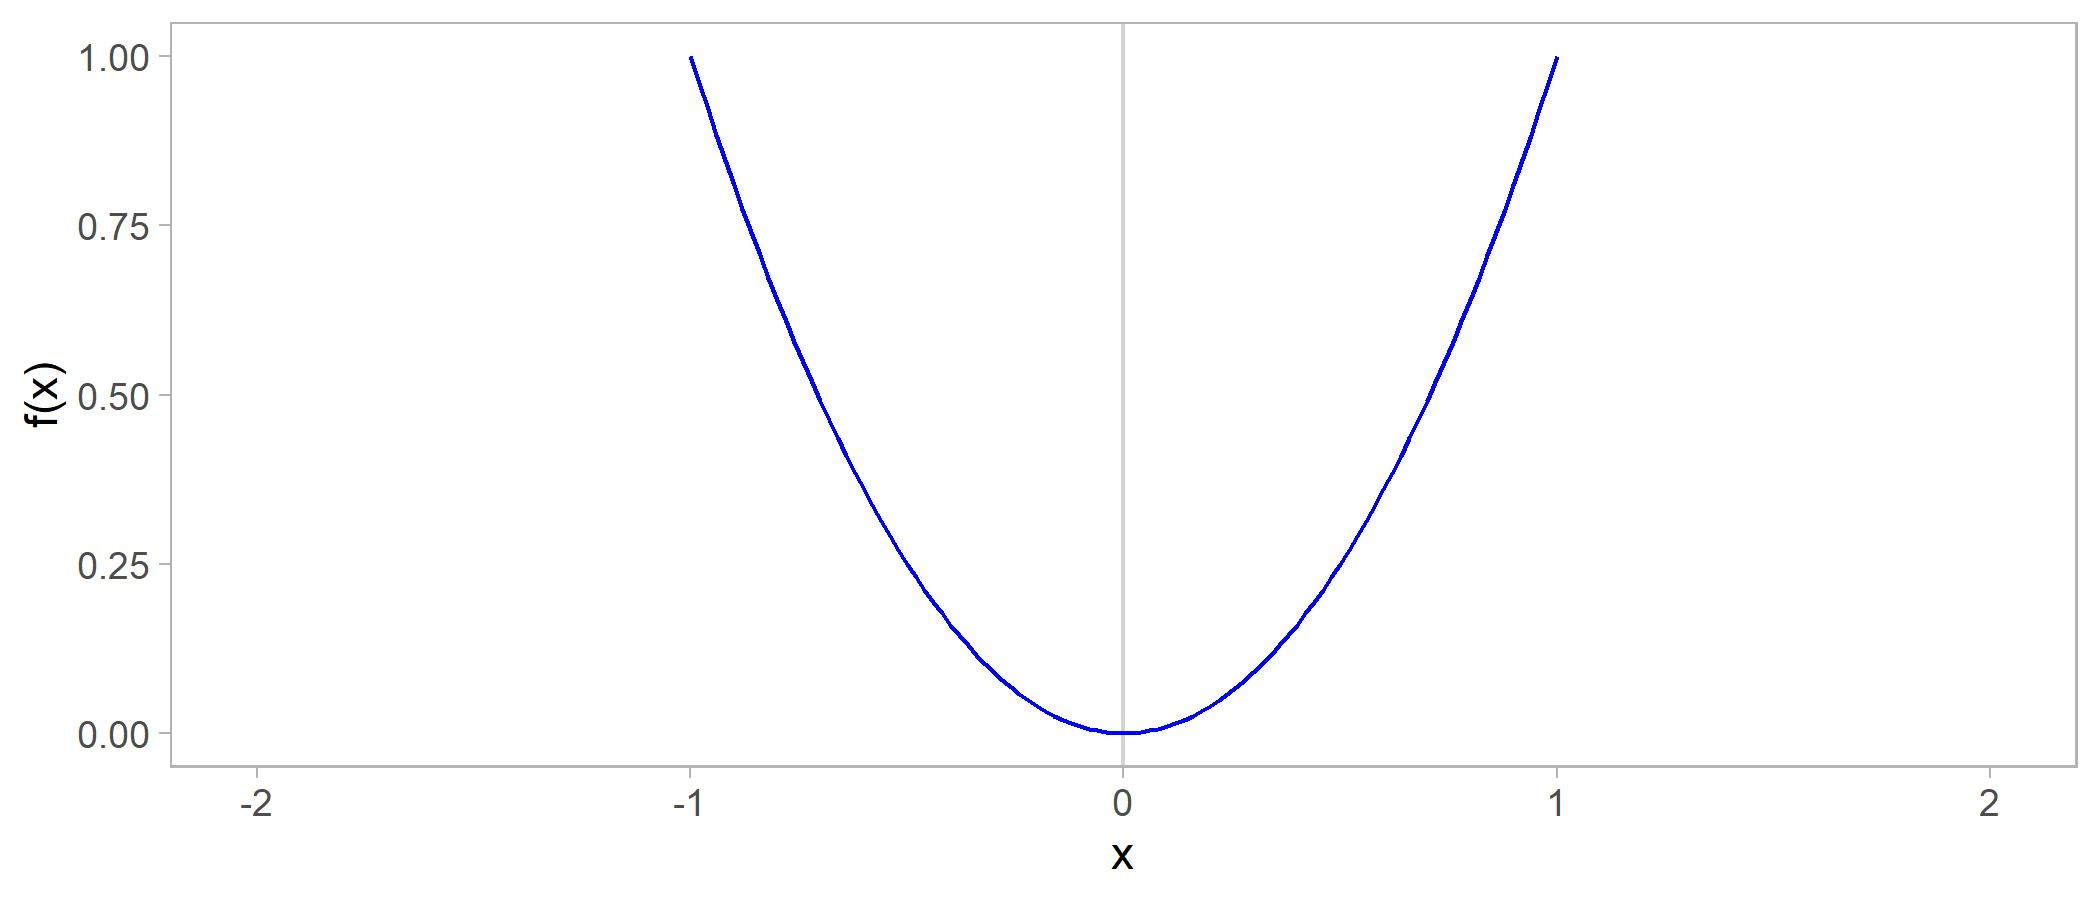
\includegraphics[scale=0.7]{img/sec_power_fun.jpg}
\end{figure}

Ahora vamos a calcular la derivada de $f(x)$ en el punto $x = 3$.
\[f'(3) = \lim_{b \to 3} \frac{f(b)-f(3)}{b-3}\]
\[f'(3) = \lim_{b \to 3} \frac{b^{2}-9}{b-3}\]
Tanto la función del numerador como del denominador, son continuas y, si establecemos $b = 3$, la fracción nos queda como $0/0$, por lo que tendremos que seguir factorizando.
\[f'(3) = \lim_{b \to 3} \frac{b^{2}-9}{b-3}\]
\[f'(3) = \lim_{b \to 3} \frac{(b+3)(b-3)}{b-3}\]
\[f'(3) = \lim_{b \to 3} b+3\]
Ahora, si reemplazamos $b = 3$ (ya que $b+3$ es una función continua), entonces:
\[f'(3) = \lim_{b \to 3} b+3\]
\[f'(3) = 6\]
Si trazamos la línea tangente en $x = 3$ (línea morada), que en este caso también corresponde a la derivada en el mismo punto, se verá de la siguiente forma:

\begin{figure}[hbt!]
\centering
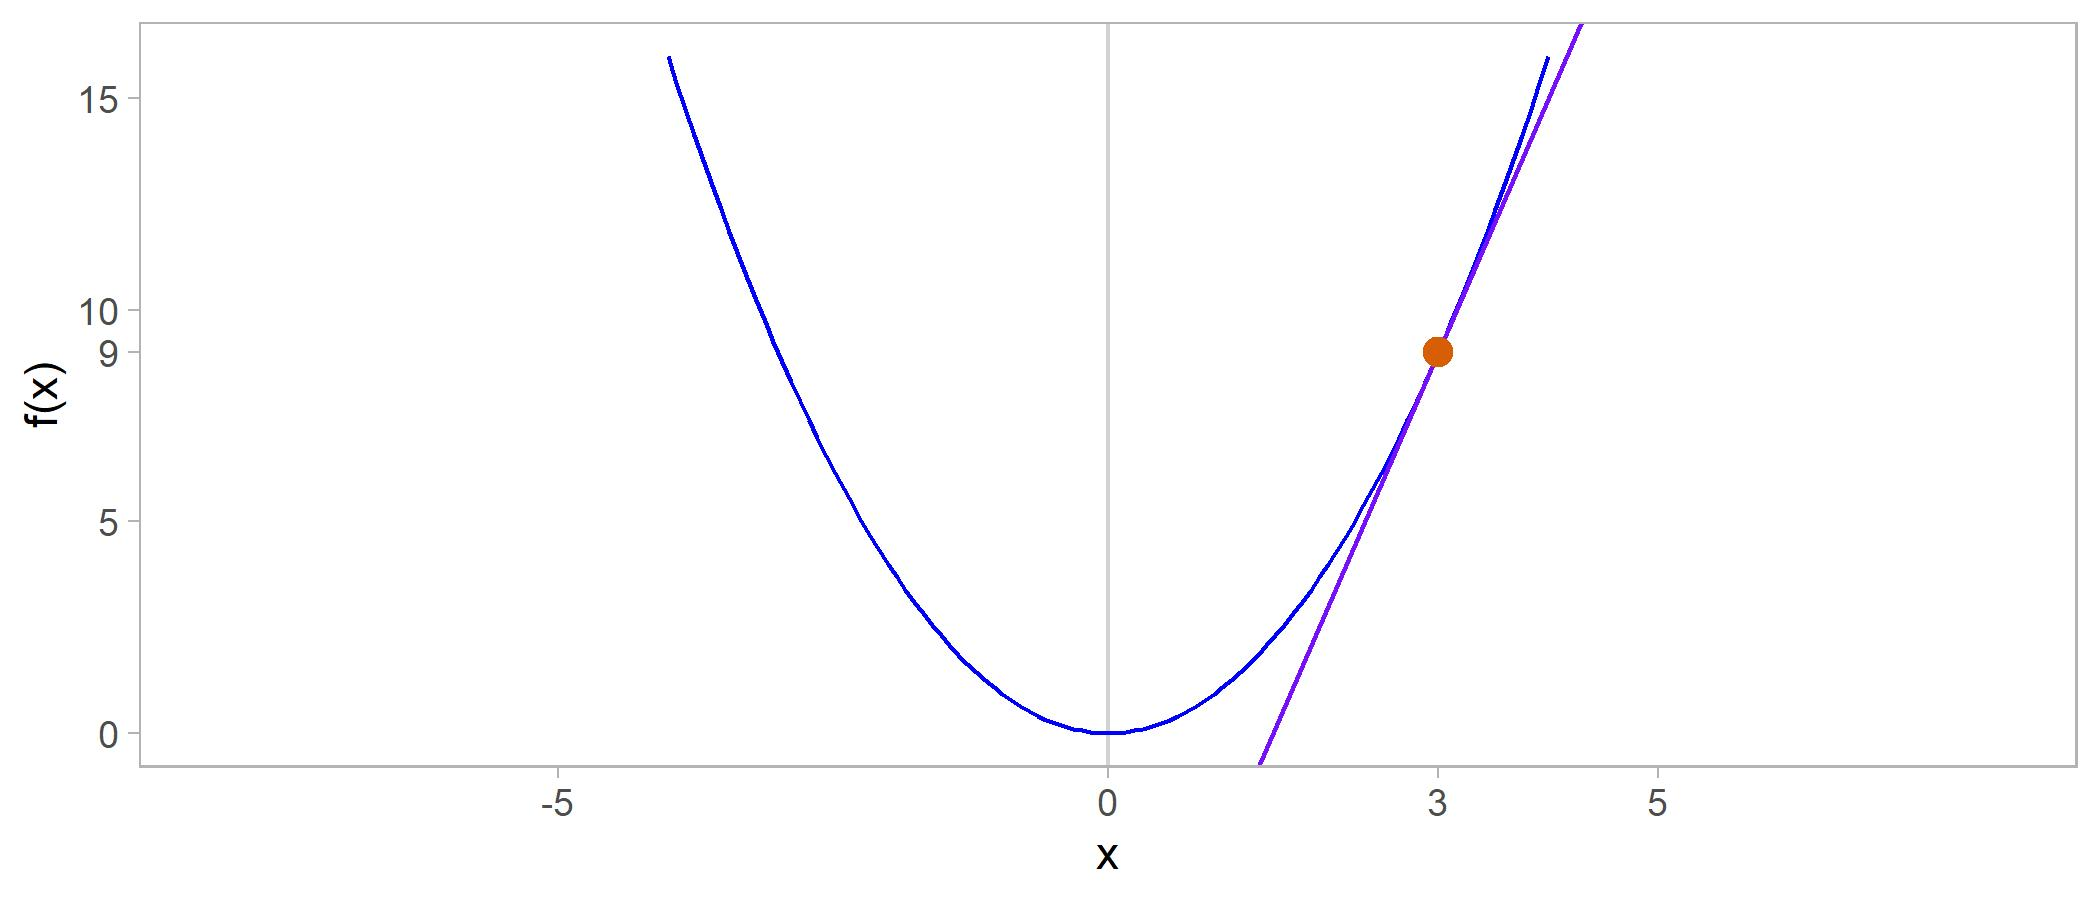
\includegraphics[scale=0.7]{img/tang_secpow_one_pt.jpg}
\end{figure}

Ahora bien, \textbf{¿qué pasaría si queremos saber las derivadas de todos los puntos de esta función ($f(x) = x^{2}$)?}

Hasta ahora, como vimos, solo sabemos que $f'(3) = 6$. De hecho, podemos visualizarla en un gráfico, en donde $f'(x) = y$, con el propósito de \textbf{ir viendo cómo se comporta en cada valor de $x$}.

\begin{figure}[hbt!]
\centering
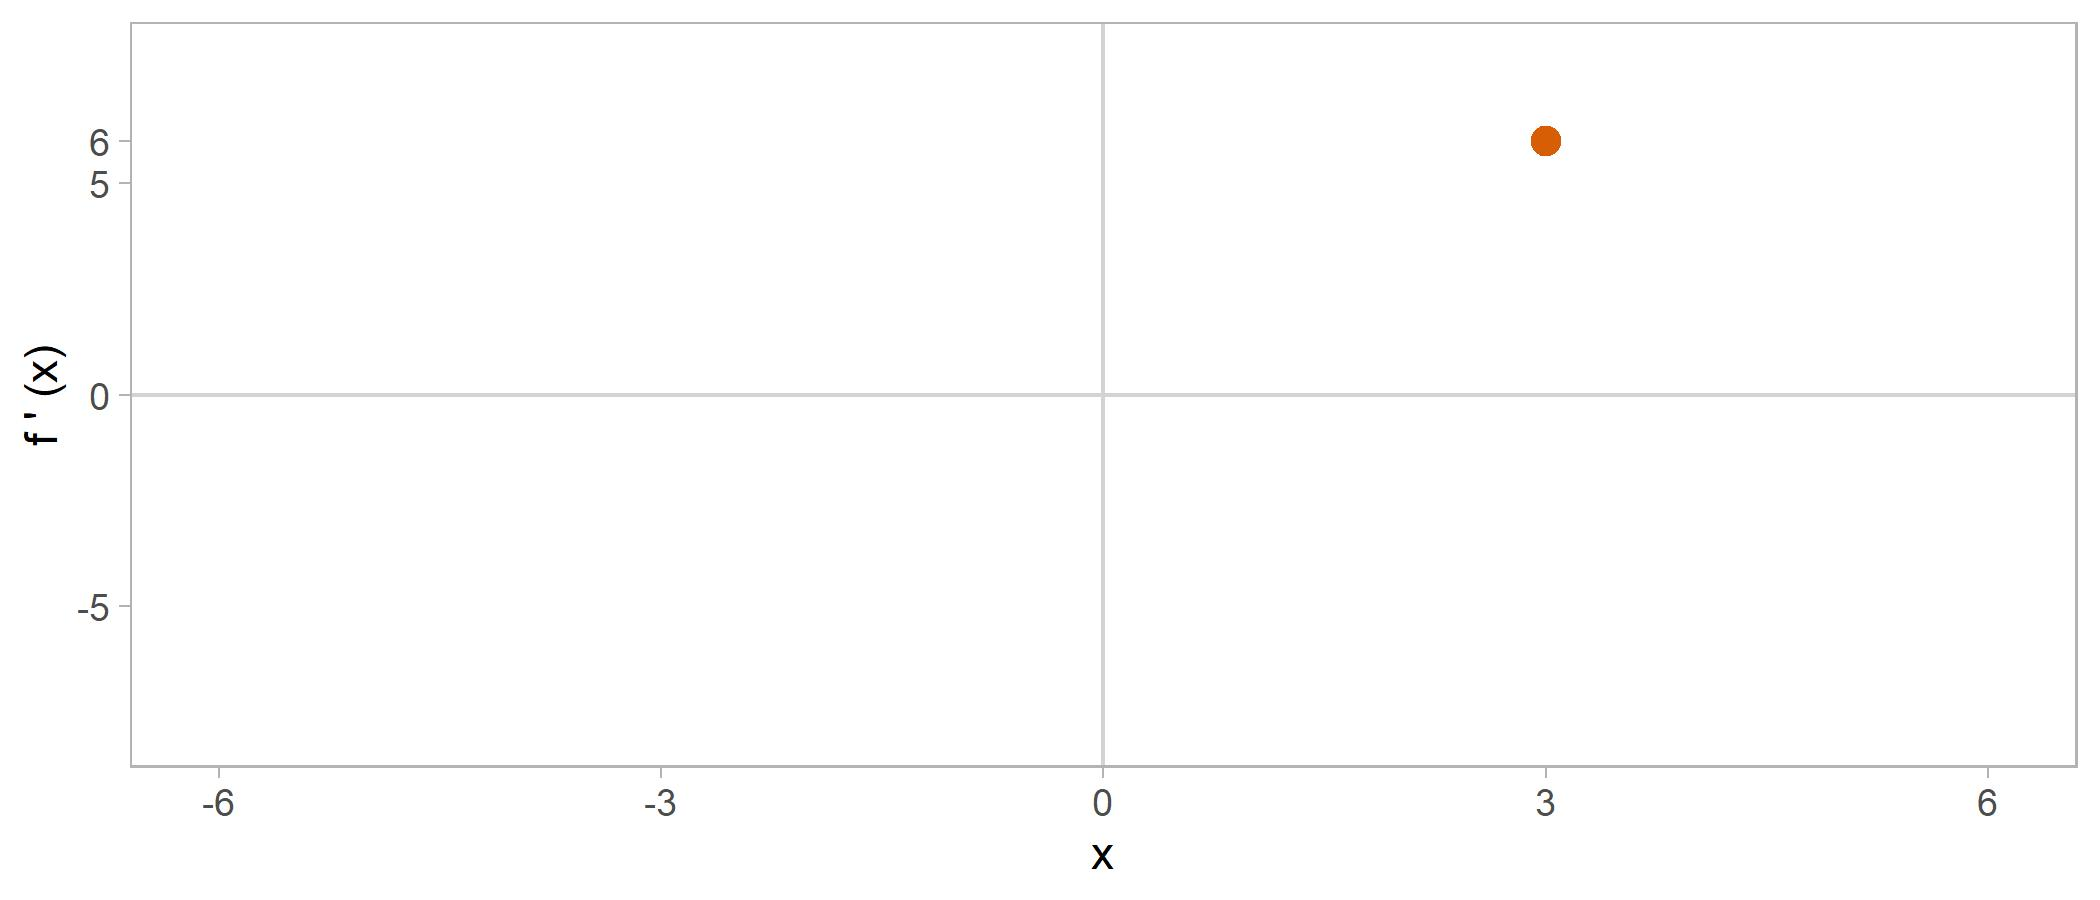
\includegraphics[scale=0.7]{img/deriv_secpow_one_pt.jpg}
\end{figure}

Sin embargo, como vemos, es bastante difícil saber cómo se comporta la derivada de la función $f(x) = x^{2}$ en cada $x$, con un solo punto. Lo ideal sería conocer las derivadas en todos los puntos, pero si aplicamos la fórmula que hemos usado hasta ahora (la tasa de cambio instantáneo) reemplazando cada valor de $x$, será una tarea muy tediosa. 

Otro camino que podemos tomar para conocer la $f(x) = x^{2}$ en todos los valores de $x$, es establecer un valor arbitrario que denominaremos como $x$, en vez de algún valor numérico (como $3$, anteriormente), y lo reemplazaremos en la fórmula de la tasa de cambio instantáneo. Es decir, diremos que:
\[f'(x) = \lim_{b \to x} \frac{f(b)-f(x)}{b-x}\]
\[f'(x) = \lim_{b \to x} \frac{b^{2}-x^{2}}{b-x}\]
\[f'(x) = \lim_{b \to x} \frac{(b+x)(b-x)}{b-x}\]
\[f'(x) = \lim_{b \to x} \, b+x\]
Si reemplazamos $b = x$, ya que $b+x$ es una función continua, entonces:
\[f'(x) = \lim_{b \to x} \, b+x\]
\[f'(x) = x+x\]
\[f'(x) = 2x\]
Por lo tanto, en vez de tener que calcular la tasa de cambio instantáneo una y otra vez para obtener las derivadas en todos los puntos de la función $f(x) = x^{2}$, podemos aplicar la fórmula $f'(x) = 2x$, que es más sencilla.

Por otra parte, la fórmula de la derivada de $f(x) = x^{2}$, que corresponde a $f'(x) = 2x$, también nos sirve para saber cómo se comporta en todos los valores de $x$.

\newpage

\begin{figure}[hbt!]
\centering
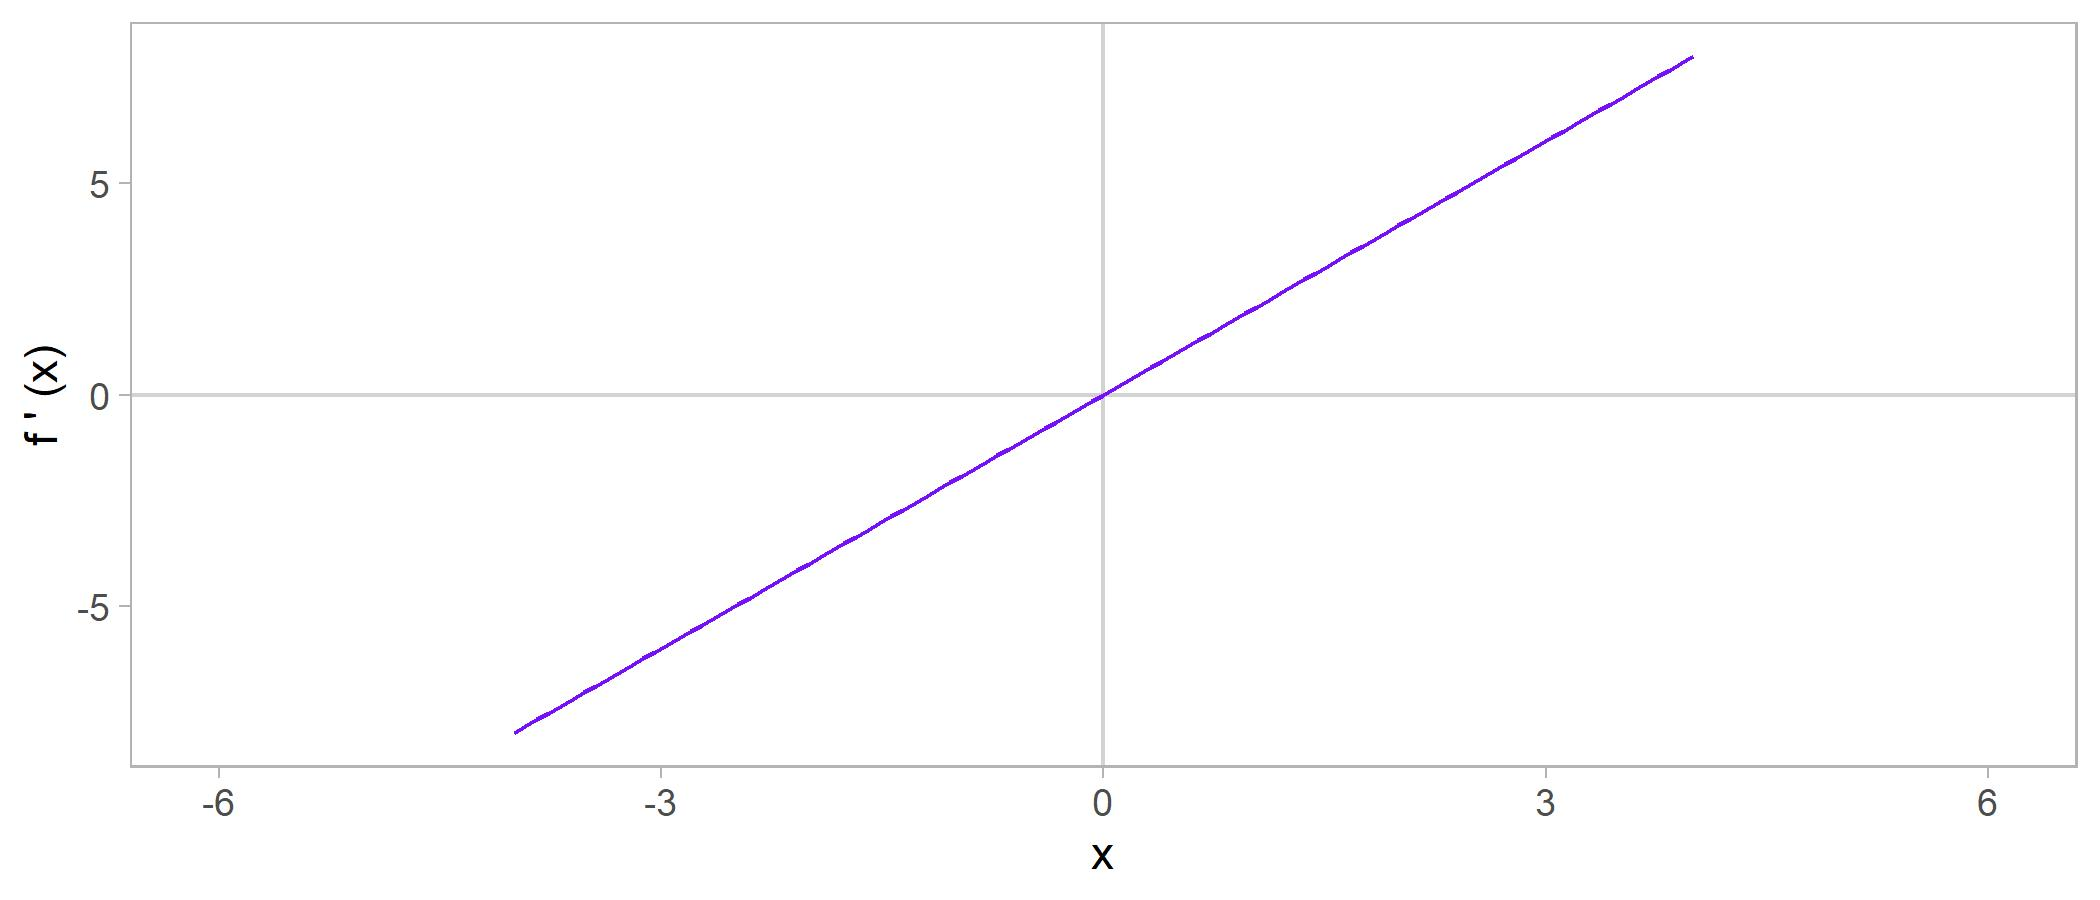
\includegraphics[scale=0.7]{img/deriv_secpow_fun.jpg}
\end{figure}

Lo que podemos interpretar de esta gráfica es que, cuando $x < 0$, las derivadas de la función $f(x) = x^{2}$ van a ser negativas. Es decir, las pendientes de las líneas tangentes de esta función van a ser negativas. Mientras que cuando $x > 0$, aquellas pendientes serán positivas. De hecho, esto último podemos ilustrarlo con $f'(3) = 6$.

\begin{figure}[hbt!]
\centering
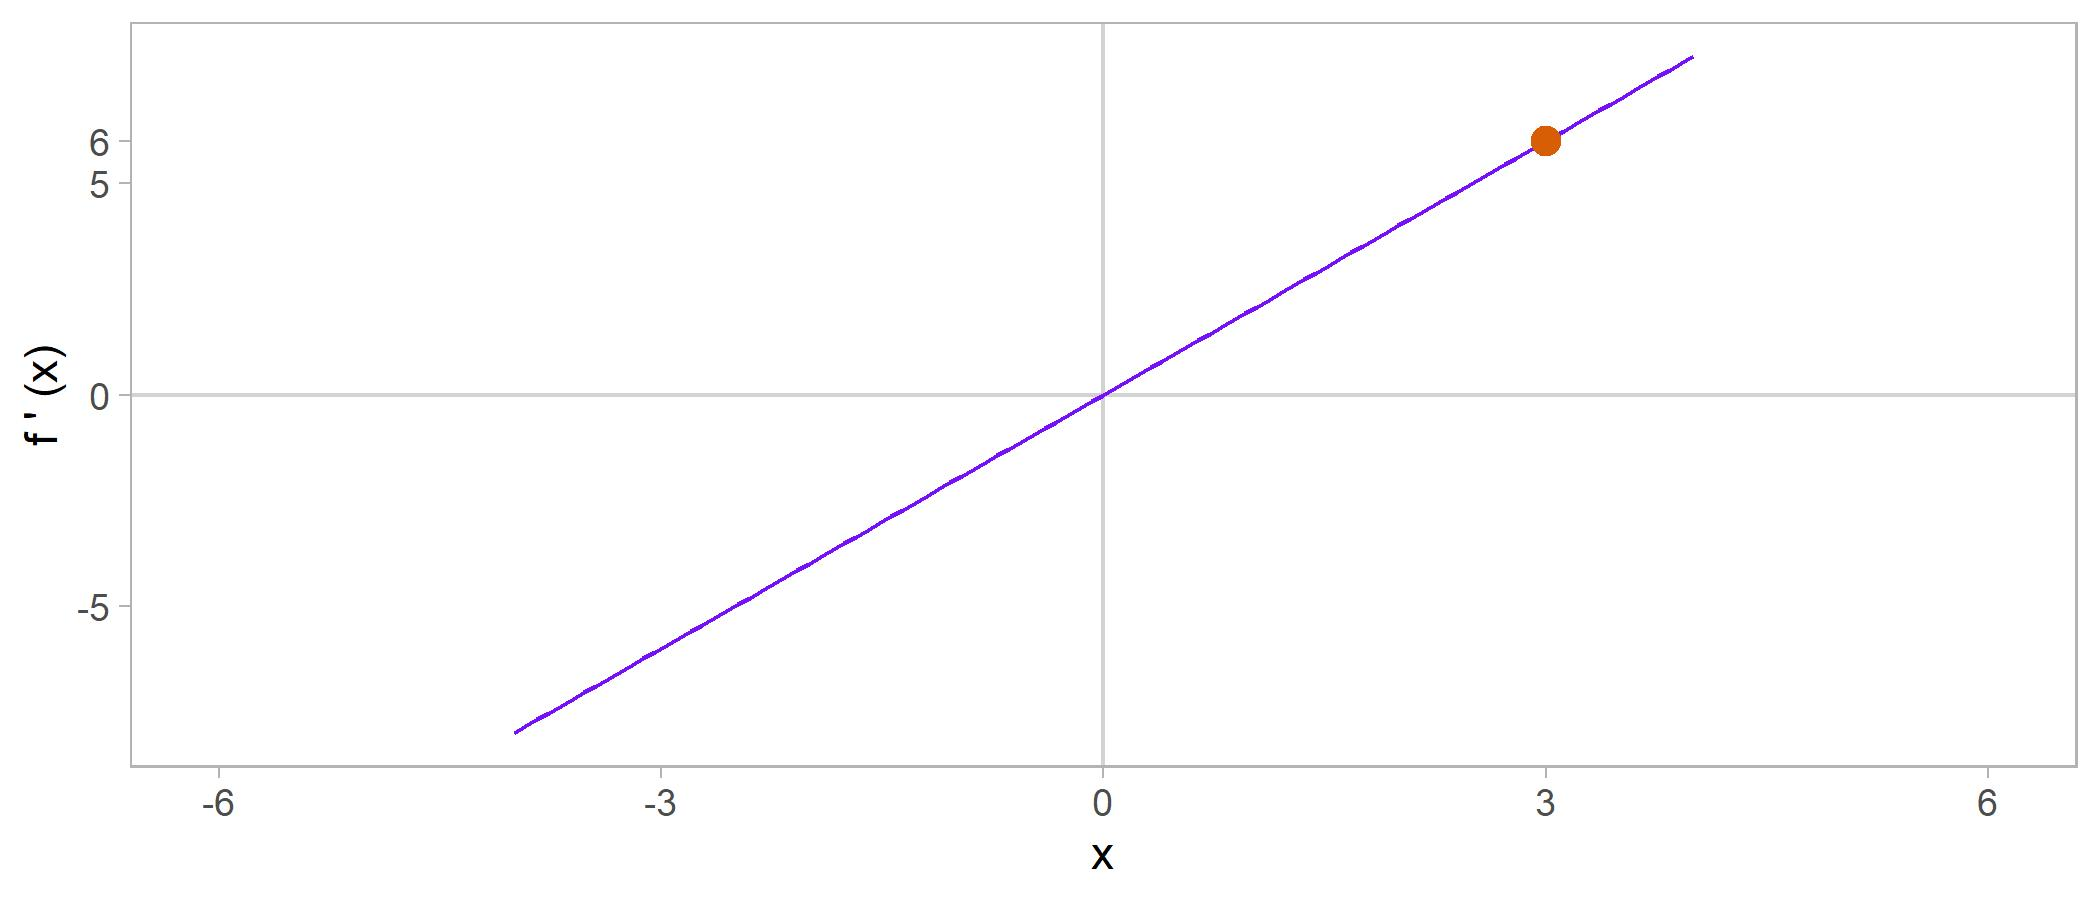
\includegraphics[scale=0.7]{img/deriv_secpow_fun_2.jpg}
\end{figure}

Para ilustrar mejor, busquémos la $f'(-2)$ de la función $f'(x) = x^{2}$ y luego dibujemos tanto la línea tangente en $f(x)$ como el punto $x = -2$ en dicha derivada.

Ahora podemos aplicar la fórmula de la derivada que encontramos antes, en vez de calcular la tasa de cambio instantánea en $x = -2$.
\[f'(-2) = 2 \cdot (-2)\]
\[f'(-2) = -4\]
Por consiguiente, la pendiente de la línea tangente de $f(x) = x^{2}$ en $x = -2$, es $-4$. Dibujémosla, así como también el punto en la gráfica de $f'(x)$.

\begin{figure}[hbt!]
\centering
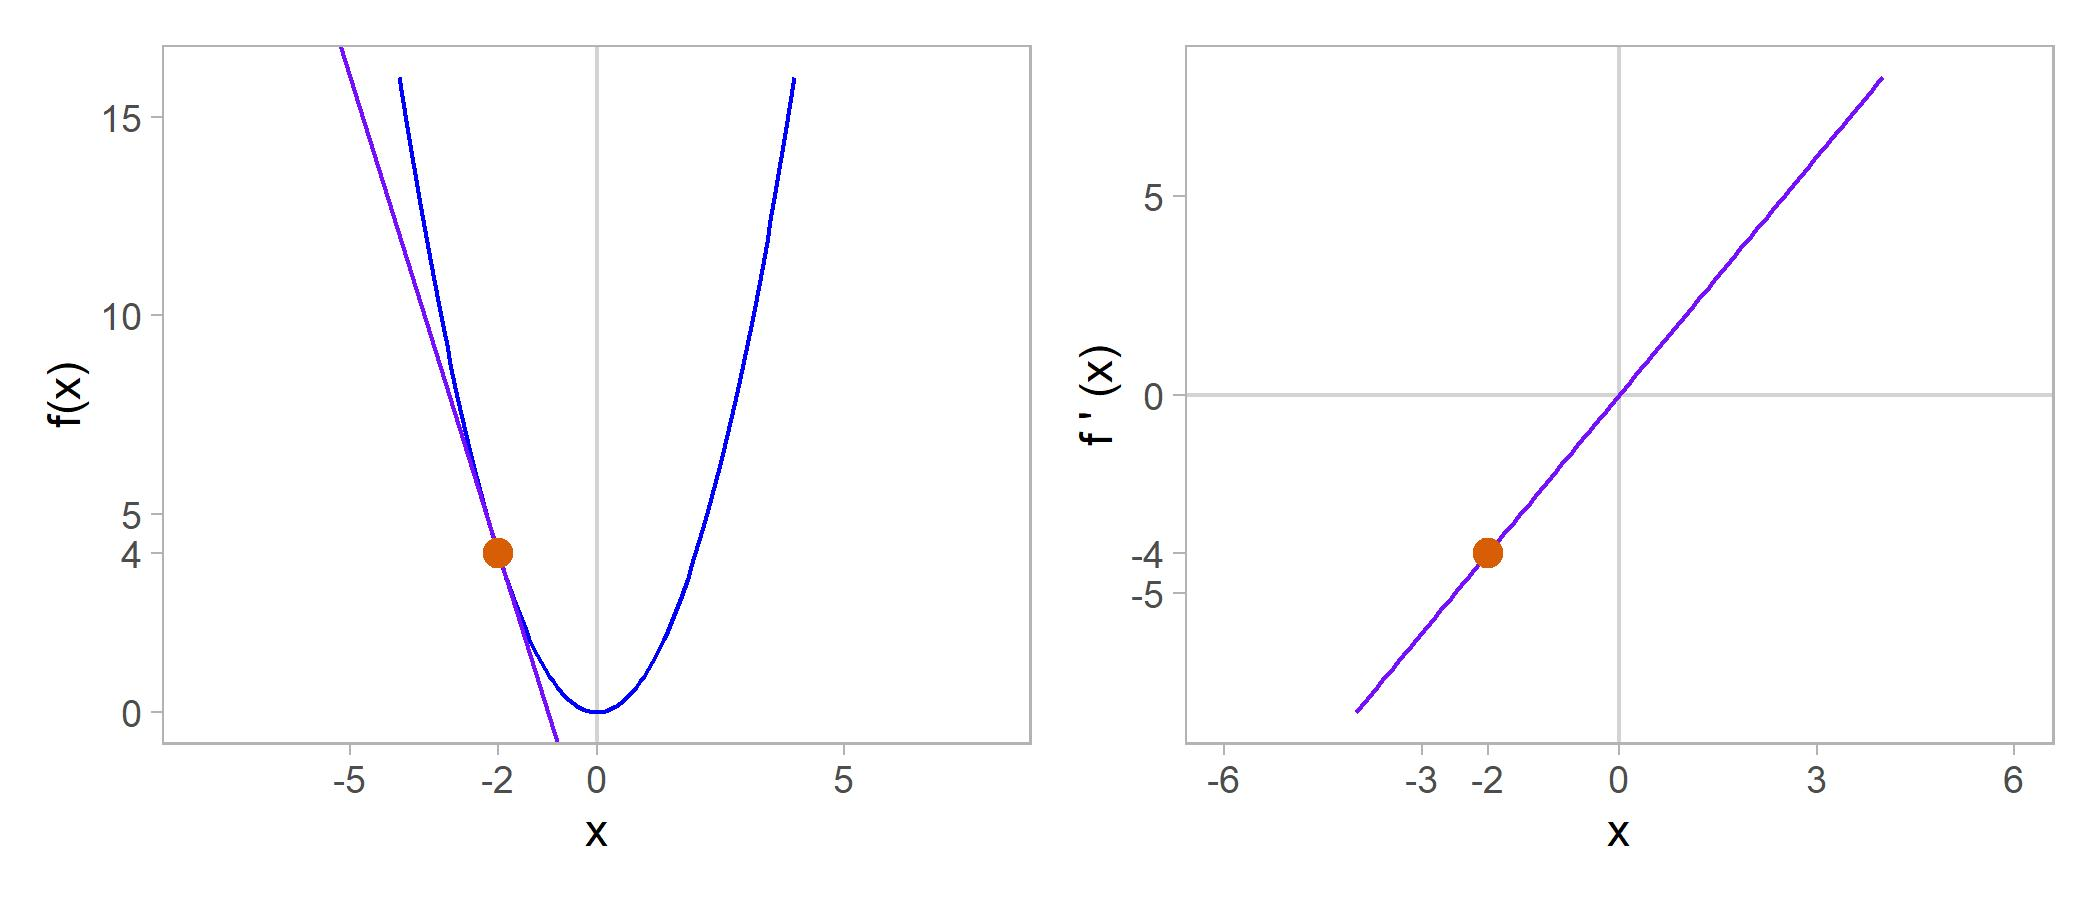
\includegraphics[scale=0.7]{img/deriv_tang_secpow.jpg}
\end{figure}

Como es posible apreciar, se cumple que la pendiente de la recta tangente en un valor $x < 0$, en la función $f(x) = x^{2}$, va a ser negativa. En este caso, la $f'(-2) = -4$.


\newpage

\subsection{Derivadas de Funciones Lineales.}

Veamos ahora la siguiente función:
\[g(x) = \frac{1}{2}x - 1\]
Su gráfica es:

\begin{figure}[hbt!]
\centering
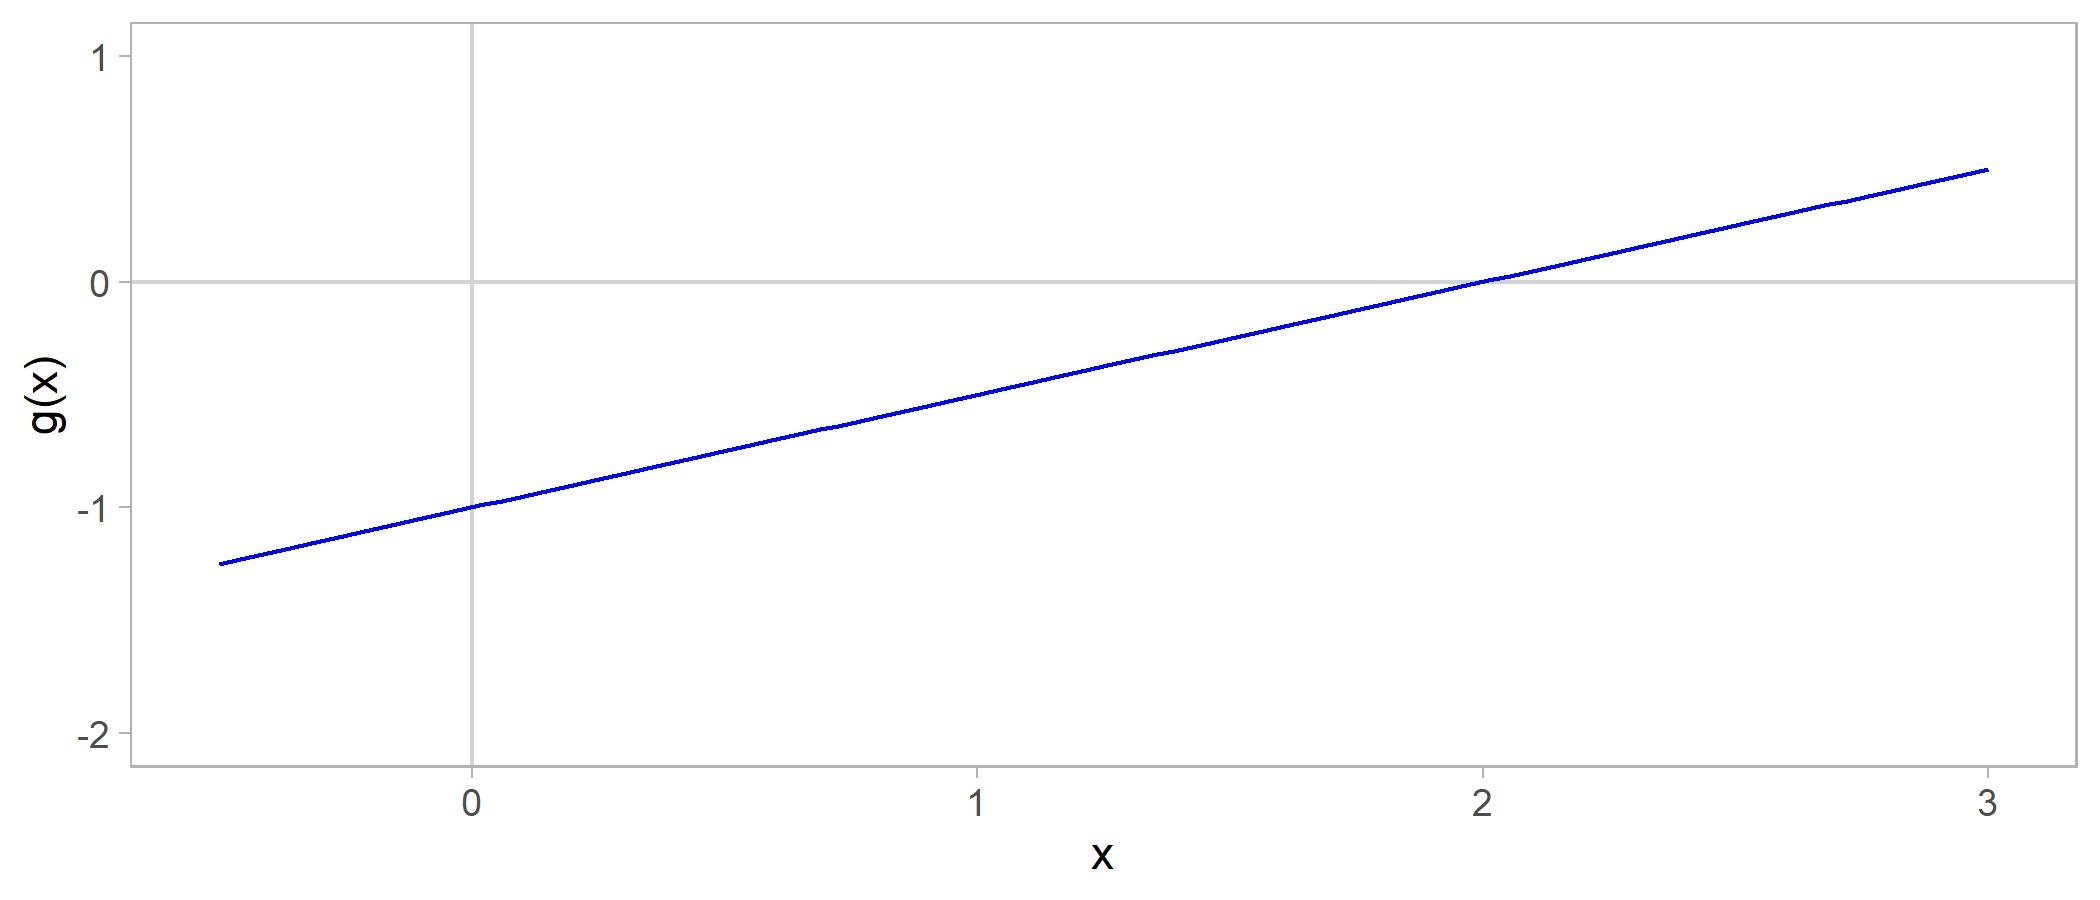
\includegraphics[scale=0.7]{img/linear_fun.jpg}
\end{figure}

Como vemos tanto en su ecuación como en su gráfica, corresponde a una \textbf{función lineal}. Una característica común de estas funciones es que sus derivadas serán iguales a sus pendientes.

Por ejemplo, busquémos la derivada de $g(x)$ en $x = 1.5$.
\[g'(1.5) = \lim_{b \to 1.5} \frac{g(b)-g(1.5)}{b-1.5}\]
\[g'(1.5) = \lim_{b \to 1.5} \frac{(0.5b-1)-(-0.25)}{b-1.5}\]
\[g'(1.5) = \lim_{b \to 1.5} \frac{(0.5b-1)-(-0.25)}{b-1.5}\]
\[g'(1.5) = \lim_{b \to 1.5} \frac{0.5b-0.75}{b-1.5}\]
\[g'(1.5) = \lim_{b \to 1.5} \frac{0.5(b-1.5)}{b-1.5}\]
\[g'(1.5) = \lim_{b \to 1.5} 0.5\]
\[g'(1.5) = 0.5 = \frac{1}{2}\]
Como vemos, la derivada en un punto $x$ de la función $g(x)$, es igual a su pendiente. Si queremos, también podemos ver la derivada en todos los valores de $x$.
\[g'(x) = \lim_{b \to x} \frac{g(b)-g(x)}{b-x}\]
\[g'(x) = \lim_{b \to x} \frac{0.5b-1-(0.5x-1)}{b-x}\]
\[g'(x) = \lim_{b \to x} \frac{0.5b-0.5x}{b-x}\]
\[g'(x) = \lim_{b \to x} \frac{0.5(b-x)}{b-x}\]
\[g'(x) = \lim_{b \to x} 0.5\]
\[g'(x) = 0.5\]
Es decir, para todos los valores de $x$, las derivadas de $g(x)$ van a ser iguales a $0.5$ ($1/2$). En ese sentido, si asumimos a $g'(x) = y$, entonces podemos señalar que va a corresponder a una \textbf{función constante}. Veamos la gráfica de $g'(x) = 0.5$.

\begin{figure}[hbt!]
\centering
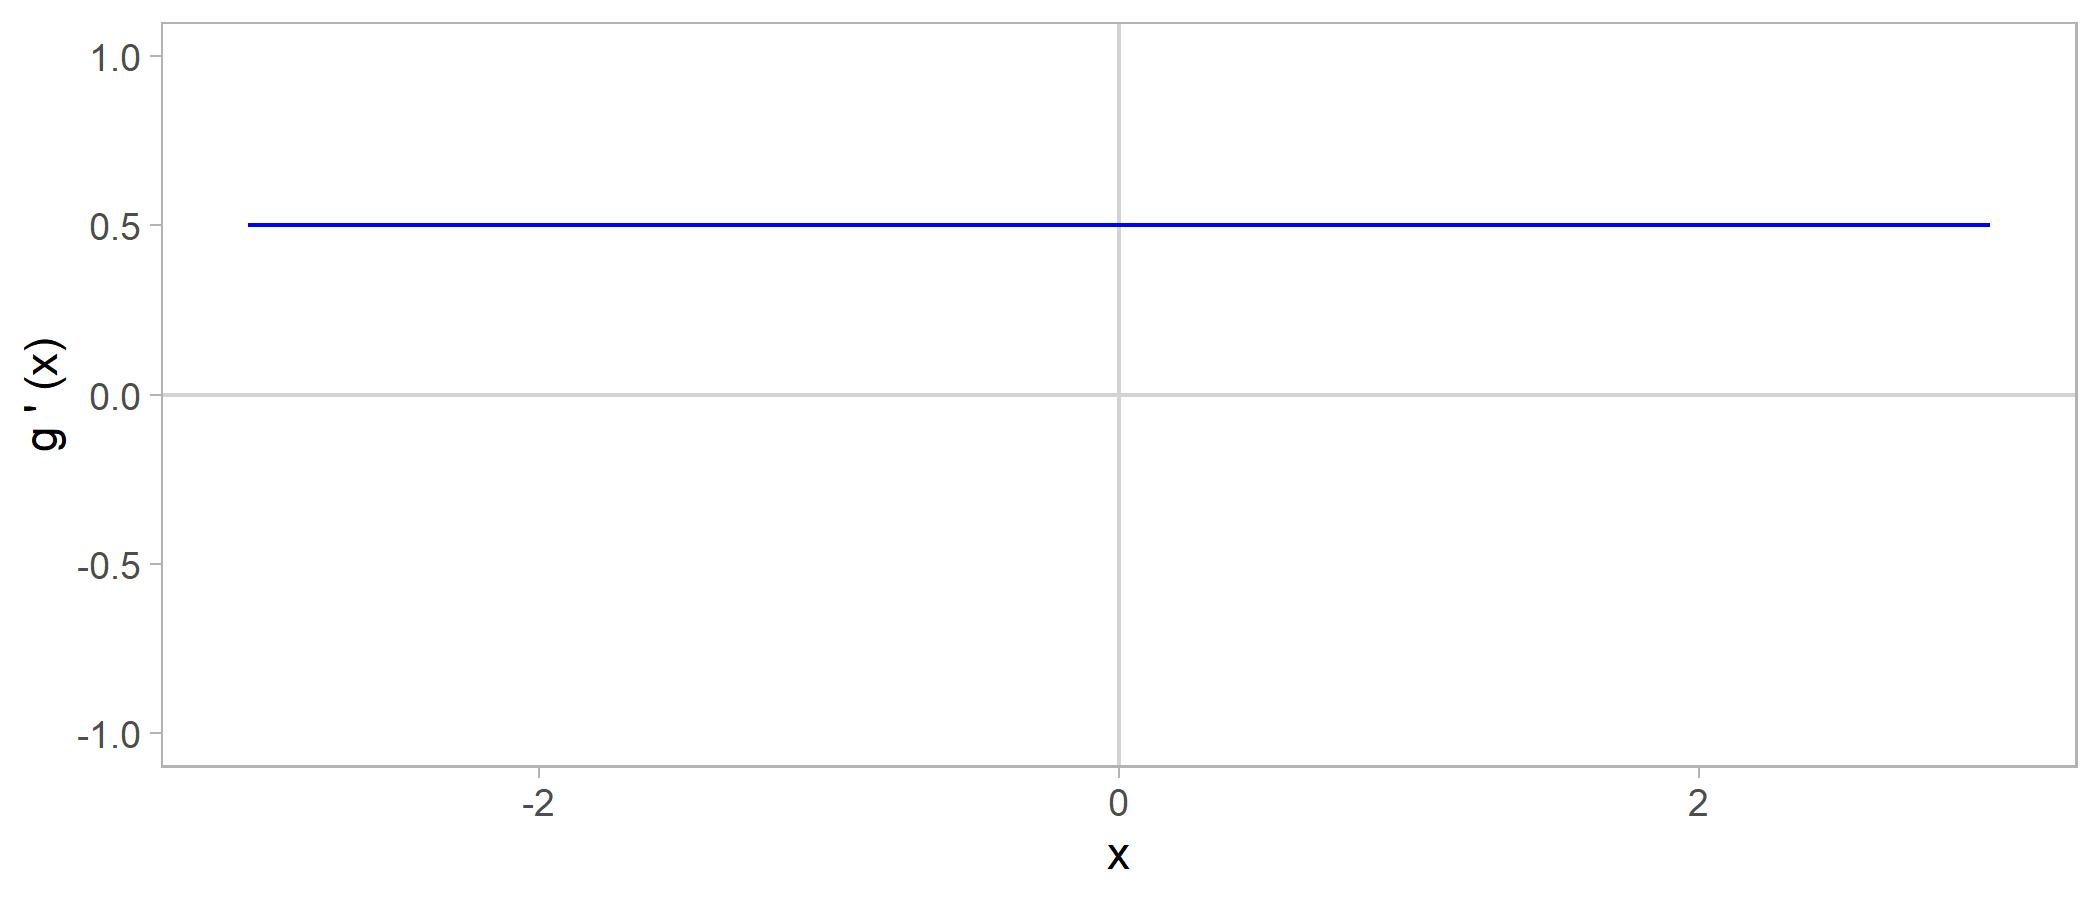
\includegraphics[scale=0.7]{img/deriv_linear_fun.jpg}
\end{figure}

En general, es posible señalar que en toda función lineal, las son del tipo $y = mx + b$, sus derivadas van a ser iguales a su pendiente. Esta afirmación la podemos demostrar algebraicamente.
\[f'(x) = \lim_{c \to x} \frac{f(c)-f(x)}{c-x}\]
\[f'(x) = \lim_{c \to x} \frac{mc+b-(mx+b)}{c-x}\]
\[f'(x) = \lim_{c \to x} \frac{mc-mx}{c-x}\]
\[f'(x) = \lim_{c \to x} \frac{m(c-x)}{c-x}\]
\[f'(x) = \lim_{c \to x} m\]
\[f'(x) = m\]
Como vemos, justamente la derivada es una constante, que corresponde a la pendiente de la función $f(x)$.

Ahora bien, \textbf{¿qué ocurre si una función lineal no tiene pendiente?} En otras palabras, si $m = 0$.

Como dijimos, las derivadas de una función lineal serán iguales a su pendiente, por lo que si $m = 0$, entonces en esta función \textbf{las derivadas serán iguales a cero}. Y, como podemos ver a continuación, éstas corresponden a las \textbf{\underline{funciones constantes}}.

Sea $m = 0$ y $f(x) = mx + b$, entonces:
\[f(x) = 0 \cdot x + b\]
\[f(x) = b\]
Por lo tanto, en las \underline{funciones constantes} las \underline{derivadas} serán \underline{iguales a cero}.

\newpage

\subsection{Notación Delta para las Derivadas.}

Hasta ahora, hemos visto que la fórmula original de una derivada es la siguiente:
\[f'(x) = \lim_{b \to x} \frac{f(b)-f(x)}{b-x}\]
Sin embargo, en ciertas ocasiones sería mejor usar una notación distinta a la de arriba.

Recordemos a qué corresponde cada parte de la fórmula de la derivada de arriba. A continuación, tenemos la curva de una función $f(x)$ (curva color morado) la cual es intersectada por una línea secante (línea color naranja) en los puntos $(x, f(x))$ y $(b, f(b))$.

\begin{figure}[hbt!]
\centering
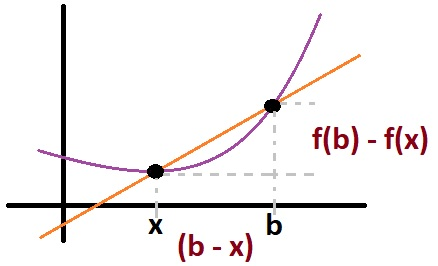
\includegraphics[scale=0.6]{img/deriv_delta_explan.jpg}
\end{figure}

Como vemos, la distancia horizontal que hay entre ambos puntos es $(b-x)$ mientras que la vertical es $f(b)-f(x)$; y la pendiente de la línea secante va a ser el cuociente entre las dos distancias antes mencionadas. Es decir:
\[m = \frac{f(b)-f(x)}{b-x}\]
Ahora bien, para esta ocasión nos vamos a concentrar en la brecha que hay entre $x$ y $b$, es decir, en $(b - x)$, y ya no en $b$. En efecto, vamos a decir que:
\[\Delta \, x = b-x\]
Este $\Delta x$ lo podemos leer como el ``cambio en $x$'' o la ``diferencia en $x$''.

Para el caso del numerador de la pendiente, lo vamos a denotar de la siguiente forma:
\[\Delta \, f = f(b) - f(x)\]
Por otra parte, vimos que $\Delta \, x = b - x$, por lo que si queremos saber cómo denotar $b$, lo podemos hacer despejando dicho valor:
\[\Delta \, x = b - x\]
\[x + \Delta \, x = x + b - x\]
\[x + \Delta \, x = b\]
Reemplacemos, por consiguiente, todos estos valores en el cálculo de la pendiente de la línea secante, que corresponde a la tasa de cambio promedio de $f(x)$:
\[m = \frac{f(b)-f(x)}{b-x}\]
\[m = \frac{f(x + \Delta \, x)-f(x)}{\Delta \, x}\]
Ahora, para conocer cuál es la derivada de $f(x)$, necesitamos saber a qué valor tiende el límite de la pendiente de la línea secante. Anteriormente vimos que, en su fórmula original, la derivada corresponde al límite de dicha pendiente, mientras  $b \to x$. No obstante, ahora estamos concentrados en $\Delta \, x$, que es igual a la diferencia entre $b$ y $x$ (i.e., $b-x$). Esto quiere decir que, \underline{a medida que $b \to x$, entonces $\Delta \, x \to 0$}, puesto que estamos diciendo que, en algún momento, $b = x$, por consiguiente:
\[\Delta \, x = b - x\]
\[\Delta \, x = x - x\]
\[\Delta \, x = 0\]
Por lo tanto, en nuestra nueva notación, la derivada de $f(x)$ también será el límite de la pendiente de la recta secante, pero mientras $\Delta \, x \to 0$. Es decir:
\[f'(x) = \lim_{\Delta \, x \to 0} \frac{f(x + \Delta \, x)-f(x)}{\Delta \, x}\]

\newpage

Usemos esta nueva notación para buscar la derivada de la función recíproca $f(x) = 1/x$.
\[f'(x) = \lim_{\Delta \, x \to 0} \frac{f(x + \Delta \, x) - f(x)}{\Delta \, x}\]
\[f'(x) = \lim_{\Delta \, x \to 0} \frac{1/(x + \Delta \, x) - 1/x}{\Delta \, x}\]
\[f'(x) = \lim_{\Delta \, x \to 0} \frac{[x - (x + \Delta \, x)]/(x + \Delta \, x)x}{\Delta \, x}\]
\[f'(x) = \lim_{\Delta \, x \to 0} \frac{x - (x + \Delta \, x)}{(x + \Delta \, x)x} \times \frac{1}{\Delta \, x}\]
\[f'(x) = \lim_{\Delta \, x \to 0} \frac{x - x - \Delta \, x}{(x + \Delta \, x)x} \times \frac{1}{\Delta \, x}\]
\[f'(x) = \lim_{\Delta \, x \to 0} \frac{- \Delta \, x}{(x + \Delta \, x)x} \times \frac{1}{\Delta \, x}\]
\[f'(x) = \lim_{\Delta \, x \to 0} \frac{-1}{(x + \Delta \, x)x} \times \frac{1}{1}\]
\[f'(x) = \lim_{\Delta \, x \to 0} \frac{-1}{(x + \Delta \, x)x}\]
Ahora bien, como podemos observar, el denominador es una función continua, por lo que podemos aplicar la propiedad:
\[\lim_{x \to a} f(x) = f(a)\]
Por lo tanto:
\[f'(x) = \lim_{\Delta \, x \to 0} \frac{-1}{(x + \Delta \, x)x}\]
\[f'(x) = \frac{\lim_{\Delta \, x \to 0} -1}{\lim_{\Delta \, x \to 0} (x + \Delta \, x)x}\]
\[f'(x) = \frac{-1}{(x + 0)x}\]
\[f'(x) = \frac{-1}{(x)x}\]
\[f'(x) = \frac{-1}{x^{2}}\]
Por consiguiente, la derivada para todos los $x$ de la función recíproca $f(x) = 1/x$, es igual a $-1/x^{2}$.



\subsection{Derivadas de Múltiplos Constantes.}

Digamos que tenemos una función $f(x)$, la cual vamos a multiplicar por 2 para obtener otra función  que denominaremos como $g(x) = 2f(x)$.

Ahora, grafiquemos ambas funciones, así como sus derivadas en el punto $x = a$.

\begin{figure}[hbt!]
\centering
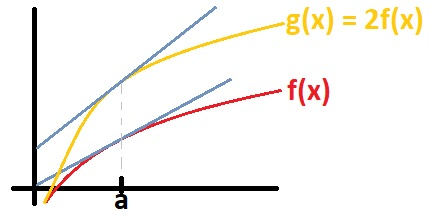
\includegraphics[scale=0.7]{img/deriv_const_mult.jpg}
\end{figure}

Como vemos, al multiplicar por 2 a $f(x)$, la función $g(x)$ se estira verticalmente al doble de $f(x)$. Y, así como se estira la función, la línea tangente en $g(x)$ se hace el doble de empinada que la correspondiente a $f(x)$. En otras palabras, podemos decir que:
\[g'(a) = 2f'(a)\]
Esto lo podemos generalizar, señalando que si, para todo $x$:
\[g(x) = kf(x)\]
entonces: 
\[g'(x) = kf'(x)\]
Veamos el siguiente ejemplo: Busquémos la derivada de $g(x) = -5x^{2}$.

Esto es lo mismo que estemos multiplicando una función $f(x) = x^{2}$, por $-5$. Es decir:
\[g'(x) = -5 \cdot (x^{2})'\]
Anteriormente (pág. 28) calculamos que la derivada de $x^{2}$ era igual a $2x$. Por lo tanto:
\[g'(x) = -5 \cdot (x^{2})'\]
\[g'(x) = -5 \cdot 2x\]
\[g'(x) = -10x\]




\subsection{Derivada de una Suma.}

Supongamos que tenemos la siguiente \underline{suma de funciones}:
\[h(x) = f(x) + g(x)\]
Entonces su derivada será:
\[h'(x) = f'(x) + g'(x)\]
Esto ocurrirá sí y solo sí, $f'(x)$ y $g'(x)$ existan.

Del mismo modo, para el caso de \underline{la diferencia} es lo mismo:

Sea:
\[h(x) = f(x) - g(x)\]
Entonces:
\[h'(x) = f'(x) - g'(x)\]
Veamos el siguiente ejemplo. Busquemos la derivada de la función $h(x)$:
\[h(x) = \frac{1}{x}+3x-7\]
Si observamos bien, tenemos dos funciones en aquella suma:
\begin{itemize}
\item Función recíproca $\rightarrow$ $1/x$
\item Función lineal $\rightarrow$ $3x-7$
\end{itemize}

Como vimos, para calcular la derivada de $h(x)$, debemos sumar las derivadas de ambas funciones que componen esa suma:
\[h'(x) = \left(\frac{1}{x}\right)' + (3x-7)'\]
Y, anteriormente, sabemos que la $(1/x)' = -1/x^{2}$ (pág. 36) y que $(3x-7)' = 3$ (pág. 31-33). Por lo tanto:
\[h'(x) = \left(\frac{1}{x}\right)' + (3x-7)'\]
\[h'(x) = \frac{-1}{x^{2}} + 3\]
Podemos demostrar algebraicamente que $h'(x) = f'(x) + g'(x)$:
\[h'(x) = \lim_{\Delta \, x \to 0} \frac{h(x + \Delta\, x) - h(x)}{\Delta \, x}\]
\[h'(x) = \lim_{\Delta \, x \to 0} \frac{[f(x + \Delta\, x) + g(x + \Delta\, x)] - [f(x) + g(x)]}{\Delta \, x}\]
\[h'(x) = \lim_{\Delta \, x \to 0} \frac{f(x + \Delta\, x) + g(x + \Delta\, x) - f(x) - g(x)}{\Delta \, x}\]
\[h'(x) = \lim_{\Delta \, x \to 0} \frac{f(x + \Delta\, x) - f(x) + g(x + \Delta\, x) - g(x)}{\Delta \, x}\]
\[h'(x) = \lim_{\Delta \, x \to 0} \frac{f(x + \Delta\, x) - f(x)}{\Delta \, x} + \frac{g(x + \Delta\, x) - g(x)}{\Delta \, x}\]
\[h'(x) = \left[\lim_{\Delta \, x \to 0} \frac{f(x + \Delta\, x) - f(x)}{\Delta \, x}\right] + \left[\lim_{\Delta \, x \to 0} \frac{g(x + \Delta\, x) - g(x)}{\Delta \, x}\right]\]
\[h'(x) = f'(x) + g'(x)\]

\newpage

\subsection{Regla de la Potencia.}

Anteriormente hemos calculado que la derivada de $f(x) = x^{2}$ es $f'(x) = 2x$ (pág. 26-30). En esta ocasión vamos a ver cómo calcular la derivada de una potencia \textbf{para cualquier exponente}. Es decir:
\[f(x) = x^{n} \Rightarrow f'(x) = ?\]
Partamos con la definición de nuestra derivada:
\[f'(x) = \lim_{b \to x} \frac{f(b) - f(x)}{b - x}\]
\[f'(x) = \lim_{b \to x} \frac{b^{n} - x^{n}}{b - x}\]
Ahora debemos factorizar el numerador y, para ello, aplicaremos la \textbf{diferencia de la n-potencia}:
\[f'(x) = \lim_{b \to x} \frac{(b - x)(b^{n-1} + b^{n-2}x + b^{n-3}x^{2} + ... + bx^{n-2} + x^{n-1})}{b - x}\]
\[f'(x) = \lim_{b \to x} \, (b^{n-1} + b^{n-2}x + b^{n-3}x^{2} + ... + bx^{n-2} + x^{n-1})\]
Esta expresión es un polinomio y sabemos que siempre son funciones continuas, por lo tanto:
\[f'(x) = x^{n-1} + x^{n-2}x + x^{n-3}x^{2} + ... + xx^{n-2} + x^{n-1}\]
Como vemos, podemos aplicar la regla de la suma de exponentes, puesto que todas las bases de las potencias son iguales:
\[f'(x) = x^{n-1} + x^{n-2+1} + x^{n-3+2} + ... + x^{1 + n-2} + x^{n-1}\]
\[f'(x) = x^{n-1} + x^{n-1} + x^{n-1} + ... + x^{n-1} + x^{n-1}\]
Podemos apreciar que todas estas expresiones son iguales a $x^{n-1}$. La pregunta que surge es ¿cuántos $x^{n-1}$ hay en total? Volvamos a la siguiente expresión:
\[f'(x) = \lim_{b \to x} \, (b^{n-1} + b^{n-2}x + b^{n-3}x^{2} + ... + bx^{n-2} + x^{n-1})\]
Es posible apreciar en el paréntesis que la cantidad de $x$ y sus exponentes van aumentando en $1$. Al inicio, tenemos $b^{n-1}x^{0}$, el cual es igual a $b^{n-1} \cdot 1 = b^{n-1}$, luego $b^{n-1}x^{1}$ y así hasta $x^{n-1}$. En otras palabras, partimos desde cero hasta $n$. Esto significa que en la expresión: 
\[f'(x) = x^{n-1} + x^{n-1} + x^{n-1} + ... + x^{n-1} + x^{n-1}\]
hay \textbf{n cantidad de veces $x^{n-1}$}. Por consiguiente, podemos decir que la derivada de $f(x) = x^{n}$, es:
\[f'(x) = n \cdot x^{n-1}\]
A esta expresión se la denomina como la \underline{\textbf{regla de la potencia}} y nos facilita el cálculo de una potencia elevada a cualquier exponente. Veamos ahora los siguientes ejemplos.

\underline{Ejemplo 1}: Calcule la derivada de $f(x) = x^{2}$.

Apliquemos la regla de la potencia para $f'(x)$:
\[f'(x) = 2 \cdot x^{2-1}\]
\[f'(x) = 2x\]
\underline{Ejemplo 2}: Calcule la derivada de $g(x) = x^{6}$:
\[g'(x) = 6 \cdot x^{6-1}\]
\[g'(x) = 6x^{5}\]

En estos dos ejemplos hemos aplicado la regla de la potencia para un exponente positivo (i.e., $n > 0$). No obstante, también podemos aplicarla a otros tipos de valores.

\underline{Ejemplo 3}: Si $f(x) = 1/x$, entonces $f'(x) =$ ¿?
\[f'(x) = \left(\frac{1}{x}\right)'\]
\[f'(x) = (x^{-1})'\]
\[f'(x) = -1(x^{-1-1})\]
\[f'(x) = -(x^{-2})\]
\[f'(x) = \frac{-1}{x^{2}}\]

\underline{Ejemplo 4}: Calcule la derivada de $g(t) = \sqrt{t}$
\[g'(t) = (\sqrt{t})'\]
\[g'(t) = (t^{1/2})'\]
\[g'(t) = \frac{1}{2}(t^{1/2 - 1})\]
\[g'(t) = \frac{1}{2}(t^{-1/2})\]
\[g'(t) = \frac{1}{2}\left(\frac{1}{t^{1/2}}\right)\]
\[g'(t) = \frac{1}{2}\left(\frac{1}{\sqrt{t}}\right)\]

Como vemos, la regla del producto tiene aplicaciones para exponentes distintos a $n > 0$. De hecho, es mejor nombrarla como \textbf{regla \underline{general} de la potencia}.

Sin embargo, a pesar de que podemos usar la regla general de la potencia en variados casos, ésta tiene sus restricciones. Podemos aplicarla sí y solo sí \textbf{el exponente es un valor fijo} y \textbf{la base es un valor variable}. Veamos algunos \underline{casos en donde no podemos aplicar esta regla}:

\begin{enumerate}
\item $f(x) = 2^{x}$ $\rightarrow$ La base está fija y el exponente es variable.
\item $g(x) = (cos \, t)^{3}$ $\rightarrow$ El exponente está fijo, pero la no es solo $t$, sino que es una función de $t$.
\item $h(x) = x^{x}$ $\rightarrow$ La base es variable, pero el exponente también lo es.
\end{enumerate}



\subsection{Notación de Leibniz.}

A lo largo de todas las anteriores secciones, hemos usado la siguiente notación para la derivada de una función $f(x)$:
\[f'(x)\]
A ésta se la denomina como la \textbf{notación de Newton}, quien es considerado como uno de los fundadores del Cálculo. Una de sus particularidades es que es bastante compacta y fácil de escribir, sobre todo cuando queremos evaluar la derivada en un valor $x$ específico. Por ejemplo, la derivada de $f(x)$ en $x = 3$ la denotamos como:
\[f'(3)\]
No obstante, simultáneamente \textbf{Gottfried Leibniz} también estaba desarrollando el Cálculo y creó su propia notación, la cual todavía es bastante usada.

Tanto la notación de Newton como la de Leibniz son comúnmente usadas en la actualidad, por lo que es importante que siempre las tengamos en mente.

Como recordaremos, cuando queremos calcular la derivada en un punto, una forma es usando la aproximación de una línea secante. Para ello, calculamos la pendiente de dicha línea en un punto $x$, a una distancia $\Delta \, x$:
\[\frac{\Delta \, y}{\Delta \, x}\]
De manera que la derivada en dicho punto $x$, corresponde al límite de la pendiente de la línea secante, a medida que $\Delta \, x \to 0$:
\[y' = \lim_{\Delta \, x \to 0} \frac{\Delta \, y}{\Delta \, x}\]
En la \textbf{notación de Leibniz}, aquella expresión la escribimos de la siguiente manera:
\[\frac{dy}{dx}\]
Prácticamente, lo que Leibniz hizo fue esconder la notación del límite de las deltas ($\Delta$) en su notación. Como recordaremos, las deltas hacen referencia a una pequeña diferencia. Por otra parte, \textbf{las ``d'' de la notación de Leibniz} corresponden a la \textbf{versión infinitesimal de aquella pequeña diferencia}. Es decir, con la ``d'' ya estamos diciendo que corresponde al ``límite de las deltas mientras $\Delta \, x \to 0$''.

La notación ``$dx/dy$'' corresponde a una de las notaciones de Leibniz. Recordemos que $\Delta \, y = \Delta \, f$, de manera que también podemos escribir la notación de Leibniz como:
\[\frac{df}{dx}\]
También, algunas personas denotan la derivada como ``algo'' que está ocurriendo con una función, por lo que la escriben como:
\[\frac{d}{dx}y = \frac{d}{dx}f\]
Finalmente, cuando queremos usar la \textbf{notación de Leibniz} para \textbf{evaluar la derivada en un valor particular de $x$}, lo hacemos de la siguiente forma. Por ejemplo, escribamos la derivada en $x = 3$:
\[\diff fx[x = 3]\]



\subsection{Derivadas de Orden Superior.}

Calculemos la derivada de $f(x) = x^{3} - 6x$:
\[f'(x) = (x^{3} - 6x)'\]
\[f'(x) = (x^{3})' - (6x)'\]
\[f'(x) = 3x^{3-1} - 6(x)'\]
\[f'(x) = 3x^{2} - 6(x^{1-1})\]
\[f'(x) = 3x^{2} - 6(x^{0})\]
\[f'(x) = 3x^{2} - 6\]
Como hemos visto en otras ocasiones, la derivada de una función la podemos interpretar como una función en sí misma. En ese sentido, podemos decir que $g(x) = f'(x)$. Por lo tanto, ahora calculemos la derivada de $g(x)$.
\[g'(x) = (3x^{2} - 6)'\]
\[g'(x) = (3x^{2})' - (6)'\]
\[g'(x) = 3(x^{2})' - 0\]
\[g'(x) = 3(2x^{2-1})\]
\[g'(x) = 3(2x)\]
\[g'(x) = 6x\]
Entonces, podemos decir que $g'(x) = 6x$ es ``la derivada de la derivada de $f(x)$''. A $g'(x)$, en realidad, se la conoce como la \textbf{segunda derivada}\footnote{En ese sentido, a $f'(x)$ también se la denomina como la \textbf{primera derivada}. Y, la primera derivada de $f(x) = x^{3} - 6x$ fue $f'(x) = 3x^{2} - 6$.} de $f(x)$ y se la denota como $f''(x)$. En ese sentido, la segunda derivada de $f(x) = x^{3} - 6x$ la escribimos como:
\[f''(x) = 6x\]
Ahora, en cuanto a la \textbf{notación de Leibniz}, anteriormente vimos que la \underline{primera derivada} la denotamos como:
\[\frac{df}{dx}\]
la que es igual a:
\[\frac{d}{dx}(f)\]
Por lo tanto, la \underline{segunda derivada} usando la notación de Leibniz se escribe como:
\[\frac{d}{dx} \left(\frac{d}{dx}(f)\right)\]
Ésta la podemos escribir de forma más compacta:
\[\left(\frac{d}{dx}\right)^{2}(f)\]
y que será lo mismo a:
\[\frac{d^{2}f}{dx^{2}}\]
Ésta última es la que más se suele usar.

Ahora, si queremos calcular la tercera derivada, en notación de Leibniz la escribiremos como:
\[\frac{d^{3}f}{dx^{3}}\]
Mientras que en notación de Newton:

\centerline{$f'''(x)$ o $f^{(3)}(x)$}




\subsection{Segunda Derivada y Concavidad de una Función.}

En cuanto a la \underline{segunda derivada}, también podemos entenderla como \textbf{una forma de medir cómo va girando o doblando una función $f$}, es decir, su \underline{concavidad}.

A continuación, al lado izquierdo tenemos un bosquejo de la gráfica de una función $f(x)$ y, a la derecha, un bosquejo de su derivada $f'(x)$.

\begin{figure}[hbt!]
\centering
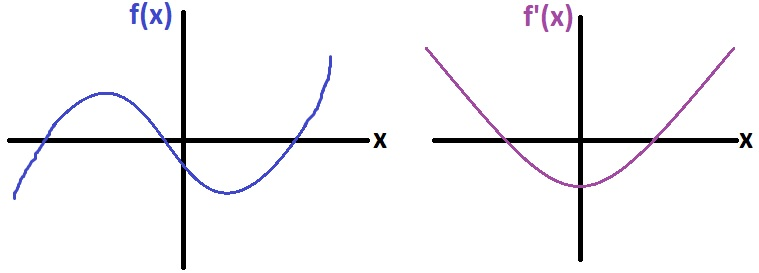
\includegraphics[scale=0.6]{img/concavity.jpg}
\end{figure}

Como vemos, si bien en el lado izquierdo de la gráfica de $f(x)$, ésta va creciendo, en la gráfica de su derivada podemos ir verificando que dicho crecimiento va siendo cada vez menor, puesto que en los mismos valores de $x$, $f'(x)$ va decreciendo a pesar de que sigue siendo positiva. Esto sigue ocurriendo hasta que $f(x)$ alcanza su valor máximo, donde su derivada $f'(x)$ es igual a cero. Quedémonos en ese punto, mientras tanto.

Ahora bien, en todo ese trayecto que acabamos de ver, cabe preguntarse \textbf{¿qué ha ido ocurriendo con la segunda derivada de $f(x)$?} Si en la gráfica de la primera derivada, $f'(x)$, en la parte que nos concentramos, trazamos las líneas tangentes en dichos valores de $x$, podemos ir viendo que en todos ellos \textbf{$f''(x)$ es negativa (i.e, $f''(x) < 0$)}. ¿Qué nos está diciendo este comportamiento de la segunda derivada $f''(x)$ con respecto a la función $f(x)$? Lo que nos va indicando es que, en aquella zona, se va formando \textbf{una curva cuya concavidad va hacia abajo}.

Del mismo modo, si seguimos avanzando en los valores de $x$ desde donde quedamos en el párrafo anterior, en algún momento la curva de la función $f(x)$ comienza a decrecer cada vez menos hasta que alcanza su punto mínimo y, luego, vuelve a crecer. Ahí, en ese mismo rango, podemos ir viendo en la gráfica de la derivada $f'(x)$ ha ido creciendo entre valores de $f'(x)$ menores a cero, igual a cero y mayores a cero (positivos) y, en dichos valores, \textbf{la segunda derivada ha ido tomando siempre valores positivos}. Esto nos indica que, en dicho rango de valores de $x$, se va formando una \textbf{concavidad hacia arriba} en la curva de la función $f(x)$.

\begin{figure}[hbt!]
\centering
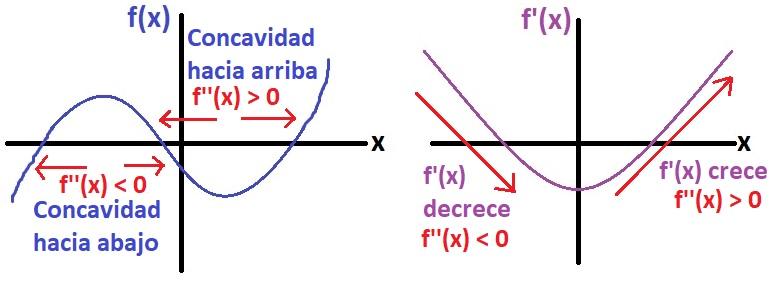
\includegraphics[scale=0.6]{img/concavity_2.jpg}
\end{figure}

En otras palabras y como se ve en la imagen de arriba, en el rango de valores en donde la derivada de la función $f(x)$ va decreciendo, las segundas derivadas van a ser negativas ($f''(x) < 0$). Esto se explicará porque, en dicho rango, la función $f'(x)$ es \textbf{concava hacia abajo}. Por otra parte, si en un rango de valores de $x$, $f'(x)$ (la primera derivada de $f(x)$) va creciendo, entonces la segunda derivada va a ser positiva ($f''(x) > 0$), porque en esa parte la función $f(x)$ es \textbf{concava hacia arriba}. De forma resumida:

\begin{itemize}
\item $f(x)$ concava hacia \underline{abajo} $\rightarrow$ $f'(x)$ es decreciente y $f''(x) < 0$.
\item $f(x)$ concava hacia \underline{arriba} $\rightarrow$ $f'(x)$ es creciente y $f''(x) > 0$.
\end{itemize}

En síntesis, como dijimos al inicio, una segunda derivada de una función $f$ nos va diciendo cómo el gráfico de dicha función va girando o doblando.

Ahora veamos el siguiente ejemplo.

\underline{Ejemplo 1}: Sea la función $f(x) = -2x^{4} + 3x^{3} + 1$, ¿cómo se verá gráficamente $f(x)$ en $x = 1$?

\underline{Respuesta}: Comencemos con calcular $f(1)$:
\[f(1) = -2(1)^4 + 3(1)^3 + 1\]
\[f(1) = -2 + 3 + 1\]
\[f(1) = 2\]

En otras palabras, sabemos que cuando $x = 1$, $f(1) = 2$.

También podemos calcular la derivada de $f(x)$:
\[f'(x) = (-2x^{4} + 3x^{3} + 1)'\]
\[f'(x) = (-2x^{4})' + (3x^{3})' + (1)'\]
\[f'(x) = -2(x^{4})' + 3(x^{3})' + 0\]
\[f'(x) = -2(4x^{3}) + 3(3x^{2})\]
\[f'(x) = -8x^{3} + 9x^{2}\]
Esto implica que $f'(1)$ es:
\[f'(1) = -8(1)^{3} + 9(1)^{2}\]
\[f'(1) = -8 + 9\]
\[f'(1) = 1\]
Con esta información tenemos conocimiento del punto $(1, 2)$ y que la pendiente de la línea tangente en dicho punto, es igual a $1$. Sin embargo, ésto no nos dice cómo será la forma de la función $f(x)$ en $x = 1$. No nos dice cómo girará o doblará y, de hecho, es un polinomio que tendrá, al menos, más de una curva. Para ello, tendremos que calcular una derivada de mayor orden, como la \underline{segunda derivada}:
\[f''(x) = (-8x^{3} + 9x^{2})'\]
\[f''(x) = (-8x^{3})' + (9x^{2})'\]
\[f''(x) = -8(x^{3})' + 9(x^{2})'\]
\[f''(x) = -8(3x^{2}) + 9(2x)\]
\[f''(x) = -24x^{2} + 18x\]
Entonces, $f''(1)$ será:
\[f''(1) = -24(1^{2}) + 18(1)\]
\[f''(1) = -24 + 18\]
\[f''(1) = -6\]
En otras palabras, la segunda derivada de $f(1)$ es $f''(1) < 0$, al menos cerca de $x = 1$. Y, como vimos en las páginas 48-49, va a implicar que en $x = 1$, la curva de $f(x)$ va a ser \textbf{cóncava hacia abajo}.




\subsection{Derivadas del Seno y del Coseno.}

A partir de lo que hemos aprendido hasta ahora sobre derivadas, vamos a aplicarlo para buscar la derivada de la función seno o $sen(x)$.

Anteriormente vimos que tanto la función seno como la función coseno, son continuas en general o para todos los $\mathbb{R}$ en $x$ (Semana 1, pág. 27). Por otra parte, su gráfica es la siguiente:

%\begin{figure}[hbt!]
%\centering
%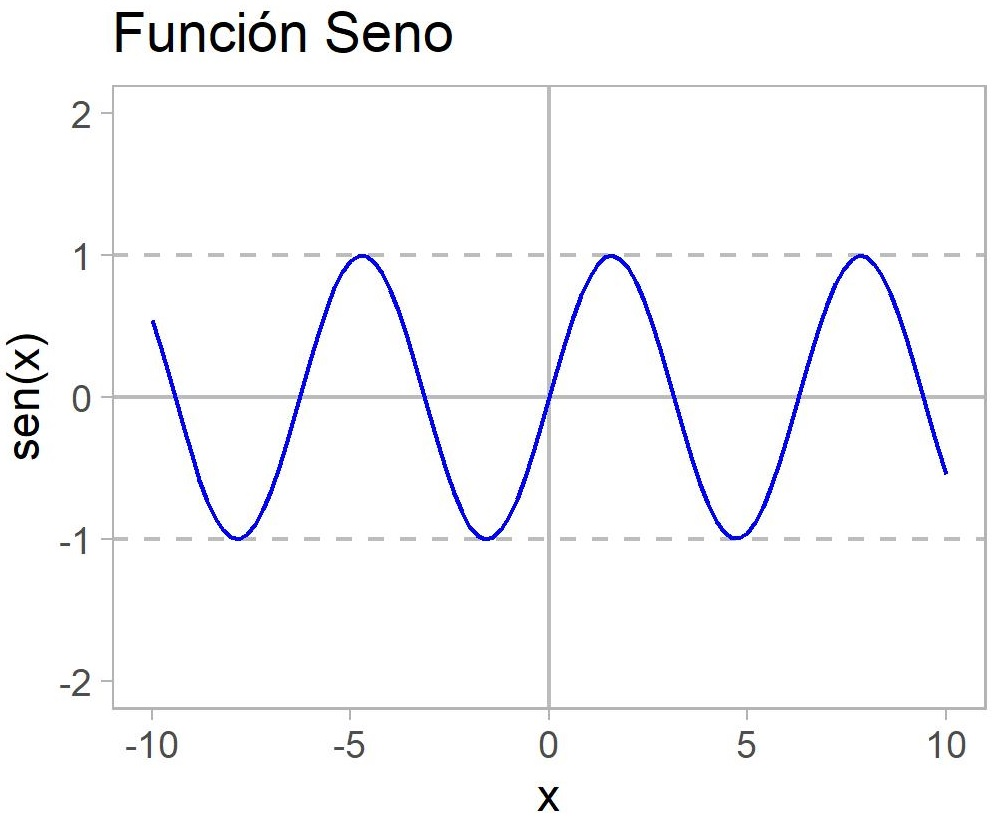
\includegraphics[scale=0.3]{img/sin_func.jpg}
%\end{figure}

De momento, la única forma que tenemos para calcular la derivada de $sen(x)$, es usando el método de la aproximación a la línea tangente, la cuál lucirá de esta manera:
\[\frac{d}{dx} sen(x) = \lim_{\Delta \, x \to 0} \frac{sen(x + \Delta \, x) - sen(x)}{\Delta \, x}\]
Como podemos ver en el numerador, tenemos la expresión $sen(x + \Delta \, x)$ la que corresponde a la \textbf{fórmula de adición para seno}:
\[sen(a + b) = sen(a) \cdot cos(b) + cos(a) \cdot sen(b)\]
Si la aplicamos al numerador de la derivada de $sen(x)$, entonces:
\[\frac{d}{dx} sen(x) = \lim_{\Delta \, x \to 0} \frac{sen(x) \cdot cos(\Delta \, x) + cos(x) \cdot sen(\Delta \, x) - sen(x)}{\Delta \, x}\]
Detengámonos un poco acá. Al inicio de esta sección señalamos que tanto la función seno como la coseno, son continuas para todos los $\mathbb{R}$ en $x$, lo cual implica que podemos aplicar la fórmula $\lim_{x \to a} f(x) = f(a)$. El problema con esto es que, cuando asumimos que $\Delta \, x = 0$, no todos los valores del numerador van a ser iguales a cero y está la posibilidad de que el límite termine siendo igual a $1/0$ que, como sabemos, su resultado no existe. La idea es que \textbf{siempre aquella fracción quede igual a $0/0$}, es por ello que un camino que podemos tomar es, primero, agrupar los términos del numerador bajo un denominador común, que en este caso es $sen(x)$ y, luego, factorizamos dicha expresión:
\[\frac{d}{dx} sen(x) = \lim_{\Delta \, x \to 0} \frac{sen(x) \cdot cos(\Delta \, x) - sen(x) + cos(x) \cdot sen(\Delta \, x)}{\Delta \, x}\]
\[\frac{d}{dx} sen(x) = \lim_{\Delta \, x \to 0} \frac{sen(x)(cos(\Delta \, x) - 1) + cos(x) \cdot sen(\Delta \, x)}{\Delta \, x}\]
y, para hacerlo más entendible, podemos separar en dos expresiones esta fracción:
\[\frac{d}{dx} sen(x) = \lim_{\Delta \, x \to 0} \frac{sen(x)(cos(\Delta \, x) - 1)}{\Delta \, x} + \frac{cos(x) \cdot sen(\Delta \, x)}{\Delta \, x}\]
\[\frac{d}{dx} sen(x) = \lim_{\Delta \, x \to 0} \left[sen(x) \left(\frac{cos(\Delta \, x) - 1}{\Delta \, x}\right) + cos(x)\left(\frac{sen(\Delta \, x)}{\Delta \, x}\right)\right]\]
De manera que terminamos obteniendo la siguiente expresión\footnote{No se explica cómo se llegó a este resultado. No obstante, tiene que ver más con una estrategia para llegar a eso. Los/as profes son del MIT, así que les creeré xd.}:
\[\frac{d}{dx} sen(x) = sen(x) \left(\lim_{\Delta \, x \to 0} \frac{cos(\Delta \, x) - 1}{\Delta \, x}\right) + cos(x)\left(\lim_{\Delta \, x \to 0} \frac{sen(\Delta \, x)}{\Delta \, x}\right)\]

Con esto, entonces, terminamos teniendo la definición de la derivada del seno y del coseno usando la aproximación a la recta tangente. Concentrémonos ahora en la derivada del seno en $x = 0$, cuya expresión es la siguiente:
\[\diff*{sen(x)}x[x = 0] = \lim_{\Delta \, x \to 0} \frac{sen(\Delta \, x)}{\Delta \, x}\]
Por el momento, no tenemos las herramientas para calcular este límite, así que tomaremos una estrategia diferente: realizaremos una \textbf{demostración geométrica} para entender la derivada de $sen(x)$.

En primer lugar, vamos a reemplazar la expresión $\Delta \, x$ por $\Theta$ (\textit{Theta}) en el límite de la expresión.
\[\diff*{sen(x)}x[x = 0] = \lim_{\Theta \to 0} \frac{sen(\Theta)}{\Theta}\]
Para la demostración vamos a usar una circunferencia unitaria (i.e., de radio $r = 1$), como la que podemos ver abajo de este párrafo. En ella, tenemos un ángulo $\Theta$ y adentro una recta vertical naranja (que, por legibilidad también la dibujamos afuera) que corresponde a $sen(\Theta)$, la cual vamos a comparar a la longitud de arco que tenemos marcado de color celeste.

\newpage

\begin{figure}[hbt!]
\centering
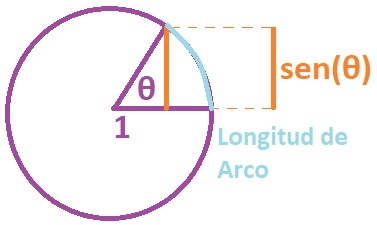
\includegraphics[scale=0.75]{img/geom_proof_sin.jpg}
\end{figure}

A partir de este punto se vuelve muy importante que el ángulo $\Theta$ sea medido en unidades de \textbf{radianes}, puesto que no servirá en grados. Esto implica que la circunferencia mide, en total, $2\pi$ que corresponde a la cantidad de radianes que hay en este círculo, lo que significa que la \textbf{longitud de arco} (color celeste) será igual a \textbf{la cantidad de radianes que son tomados por el ángulo $\Theta$}. Es decir, \textbf{la longitud de arco que vemos en la imagen de arriba es exactamente igual a $\Theta$}.

Entonces, lo que estamos intentando entender es la derivada del $sen(\Theta)$, que va a corresponder a la razón de la línea vertical (color naranjo) a la longitud del arco (color celeste), a medida que $\Theta$ se acerca a cero, es decir, a medida que dicho ángulo se va cerrando cada vez más.

Y bueno, a medida que el ángulo $\Theta$ va cerrándose (i.e., a medida que $\Theta \to 0$), si hicieramos un zoom en la circunferencia, podríamos ver que la longitud de arco (color celeste) va haciéndose cada vez más vertical y va asemejándose a la línea vertical de color naranjo, que corresponde al $sen(\Theta)$, por tanto va acercándose al valor del radio de esta circunferencia, que es igual a 1. Por lo tanto, a medida que $\Theta \to 0$, la derivada de $sen(\Theta)$ $\to 1$. Es decir, el límite que vimos en la fórmula de esta derivada, es igual a 1:
\[\diff*{sen(\Theta)}\Theta[\Theta = 0] = \lim_{\Theta \to 0} \frac{sen(\Theta)}{\Theta}\]
\[\diff*{sen(\Theta)}\Theta[\Theta = 0] = 1\]
La enseñanza es que las líneas curvadas son, esencialmente, líneas rectas cuando se les aplica zoom.

Ahora bien, como dijimos, hemos realizado esta demostración asumiendo que el ángulo es medido en radianes. En esta ocasión veremos por qué solo ahí hace sentido, pero en la realidad no lo hace.

Lo que vimos en esta derivada fue la pendiente de la recta tangente a medida que $\Theta \to 0$, cuyo ángulo está en radianes. Veamos su gráfica.

\begin{figure}[hbt!]
\centering
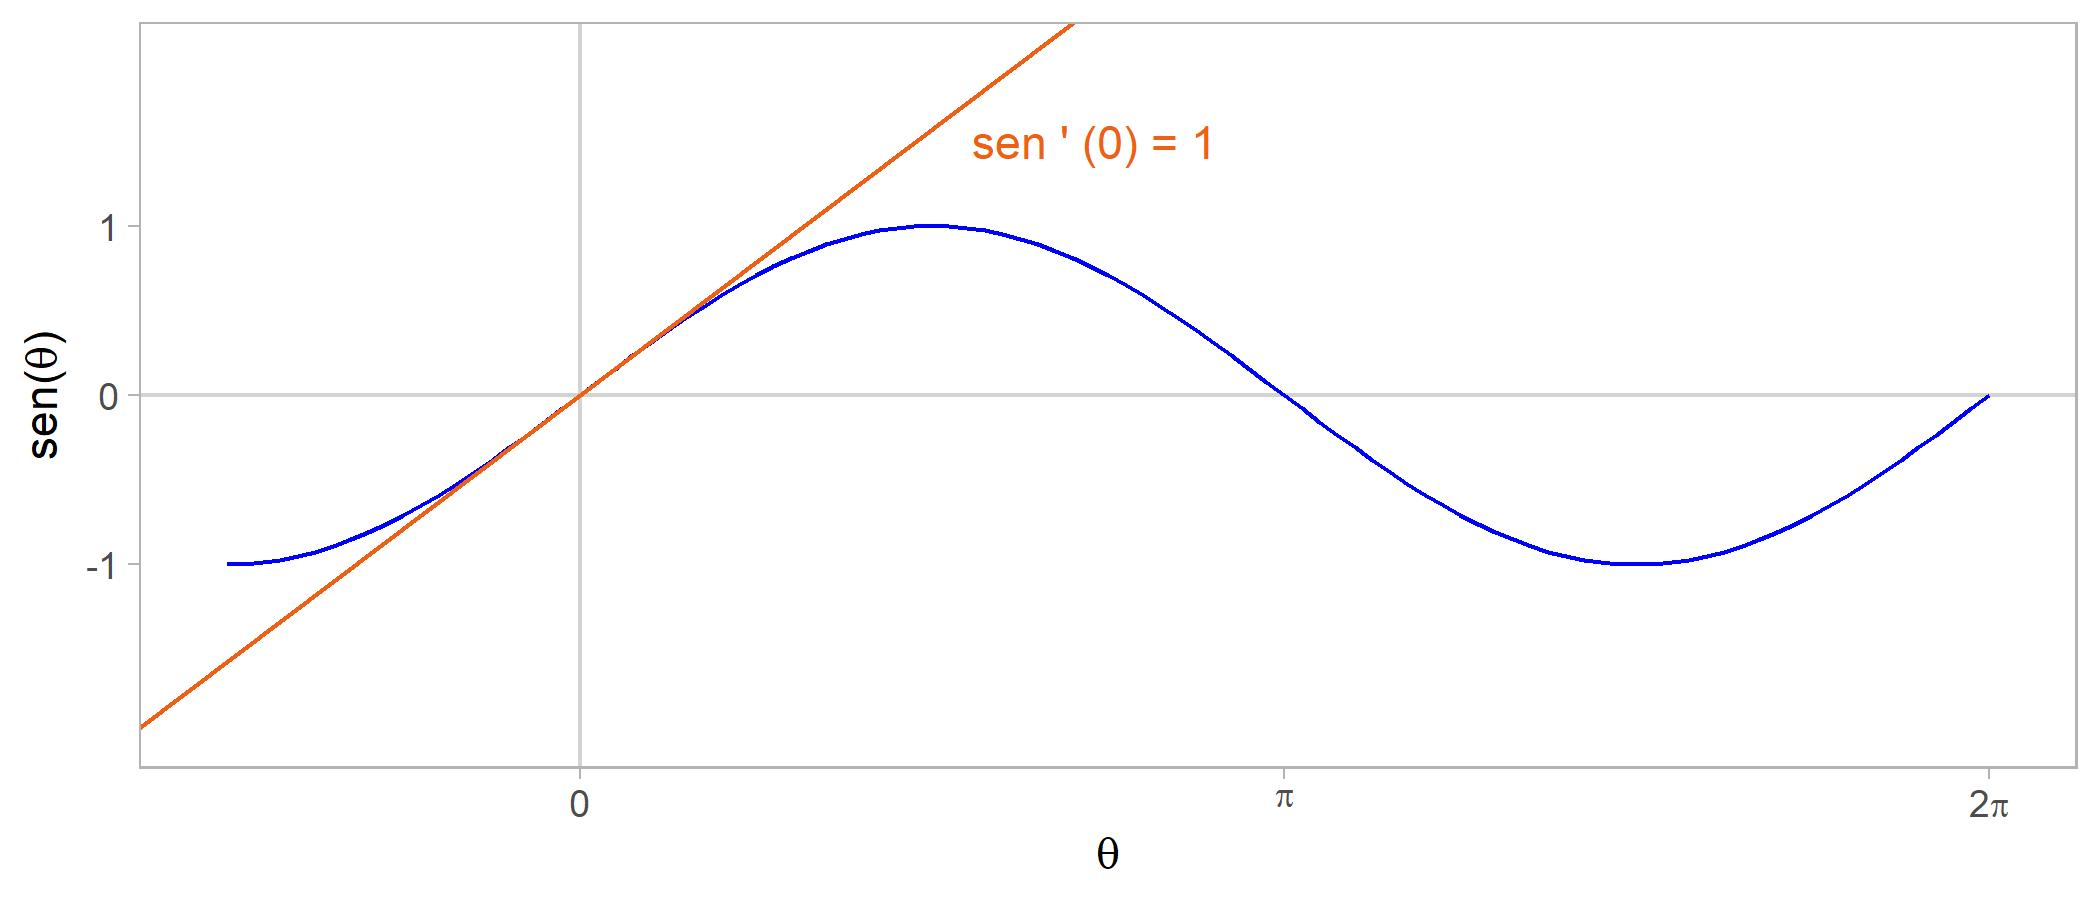
\includegraphics[scale=0.7]{img/deriv_sin_theta.jpg}
\end{figure}

Ahora bien, si pasamos a \underline{medir dicho ángulo en grados}, entonces el resultado de la derivada de $sen(\Theta)$ no tiene sentido. De hecho, si la graficamos\footnote{No supe cómo replicar este gráfico en R, así que le saqué un pantallazo al video del curso, el cual es un bosquejo pero no muy distinto a cómo sería realmente.} podemos ver que ahora es distinto a 1. Las curvas de la función $sen(\Theta)$ es más aplanada y su derivada en $\Theta = 0$ también lo es.

\begin{figure}[hbt!]
\centering
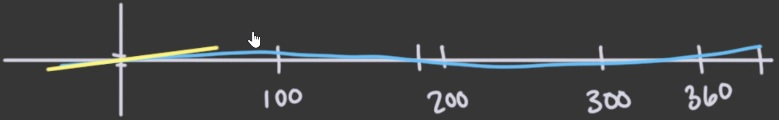
\includegraphics[scale=0.7]{img/deriv_sin_degrees.jpg}
\end{figure}

Por lo tanto, \textbf{la derivada de $sen(\Theta)$ en $\Theta = 0$ es solo igual a $1$ si $\Theta$ es medido en \underline{radianes}}.


Ahora nos concentraremos en la demostración geométrica de la derivada del \underline{coseno}.
\[\frac{d}{dx}cos(x) = \lim_{\Delta \, x \to 0} \frac{cos(\Delta \, x) - 1}{\Delta \, x}\]
Del mismo modo a como lo hicimos con la derivada del seno, también reemplazaremos $\Delta \, x$ con $\Theta$, que corresponderá al ángulo.
\[\frac{d}{d\Theta}cos(\Theta) = \lim_{\Theta \to 0} \frac{cos(\Theta) - 1}{\Theta}\]
También usaremos la imagen de una circunferencia unitaria (i.e., $r = 1$), donde tendremos el $\angle \, \Theta$ (ángulo \textit{theta}), el $sen(\Theta)$ (línea vertical naranja), la longitud de arco que es igual a $\Theta$ (arco color celeste).

\begin{figure}[hbt!]
\centering
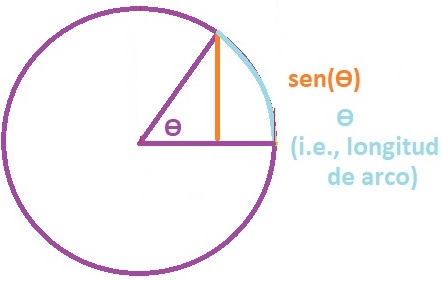
\includegraphics[scale=0.7]{img/geom_proof_cos.jpg}
\end{figure}

Como vemos en la fórmula de la derivada del $cos(\Theta)$, lo que necesitamos conocer es el numerador $cos(\Theta) - 1$. Como dijimos, esta es una circunferencia unitaria, por tanto y como podemos ver en la imagen de abajo, la distancia entre el centro de ésta y su arco es igual a 1 o, en otras palabras, $r = 1$ (línea horizontal roja). 

\newpage

\begin{figure}[hbt!]
\centering
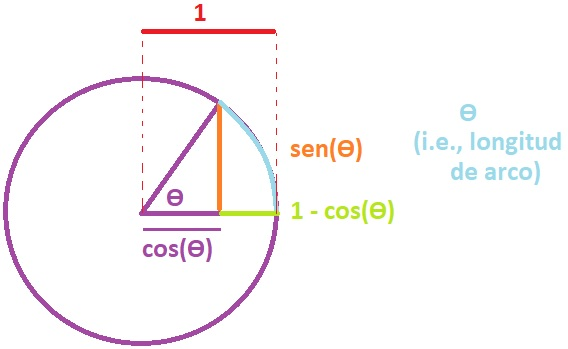
\includegraphics[scale=0.7]{img/geom_proof_cos_1.jpg}
\end{figure}

En ese sentido, la distancia que se crea entre la base del triangulo formado por la línea vertical (naranja) con el radio, corresponde al $cos(\Theta)$ y, por consiguiente, el resto de dicho radio (color verde) será igual a $1 - cos(\Theta)$. Como podemos apreciar, éste último corresponde al valor negativo del numerador del límite, $cos(\Theta) - 1$. No hay problema en que sea negativo, ya que al final de su cálculo se puede cambiar su signo. Además, el valor $1 - cos(\Theta)$ nos permite calcular distancias positivas de forma más fácil.

Ahora bien, estamos interesados en ver qué ocurre cuando $\Theta \to 0$. Para esto, vamos a mantener constante el $sen(x)$ (i.e., no lo achicaremos) y, para disminuir el ángulo hacia cero vamos a alargar el radio de la circunferencia unitaria, lo que implica que el tamaño de ésta aumentará también. Veamos una parte de este proceso.

\newpage

\begin{figure}[hbt!]
\centering
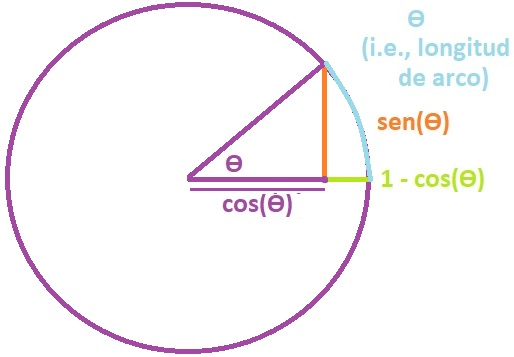
\includegraphics[scale=0.7]{img/geom_proof_cos_2.jpg}
\end{figure}

Como podemos observar, al achicarse el $\angle \Theta$ (i.e., a medida que $\Theta \to 0$) producto de haber alargado el radio de la circunferencia unitaria, el valor de $1 - cos(\Theta)$ también va haciéndose más pequeño. 

Anteriormente señalamos que mientras $\Theta \to 0$, entonces $sen(\Theta) \approx \Theta$ y, por consiguiente, ambos a su vez se acercan a cero ($sen(\Theta)$ y $\Theta$ $\to 0$) (pág. 53). Del mismo modo, cuando $\Theta \to 0$, el valor de $1 - cos(\Theta)$ también se acerca a cero, pero lo hace más rápido que lo hacen el $sen(\Theta)$ y $\Theta$. Esto lo podemos observar en la imagen de arriba, donde con solo haber disminuido un poco el $\angle \Theta$, el valor de $1 - cos(\Theta)$ se acercó en mayor magnitud a cero (se achicó más). Lo que nos está diciendo esto es que el numerador del límite que usamos para calcular la derivada del $cos(\Theta)$ va achicándose más rápido mientras $\Theta \to 0$, en comparación a cómo lo hace el denominador, lo que implica que \textbf{el numerador se va a igualar a cero más rápidamente que el denominador, por lo que aquella división siempre va a ser igual a cero}\footnote{Cero dividido por cualquier valor, siempre será igual a cero.}.

\newpage

Veamos si la demostración geométrica que hicimos con respecto a que el numerador del límite para calcular la derivada del $cos(\Theta)$ se acerca a cero más rápidamente, llevando a que la derivada sea igual cero, hace sentido. Recordemos que hemos identificado dicho límite como la derivada en $x = 0$.
\[\diff*{cos(\Theta)}\Theta[\Theta = 0] = \lim_{\Theta \to 0} \frac{cos(\Theta) - 1}{\Theta}\]
\[\diff*{cos(\Theta)}\Theta[\Theta = 0] = 0\]
Esto debiera significar que si graficamos la curva de la función $cos(\Theta)$ y agregamos la recta tangente en $x = 0$, ésta debiera ser una línea horizontal (i.e., la primera derivada debe ser una función constante). Veamos aquello.

\begin{figure}[hbt!]
\centering
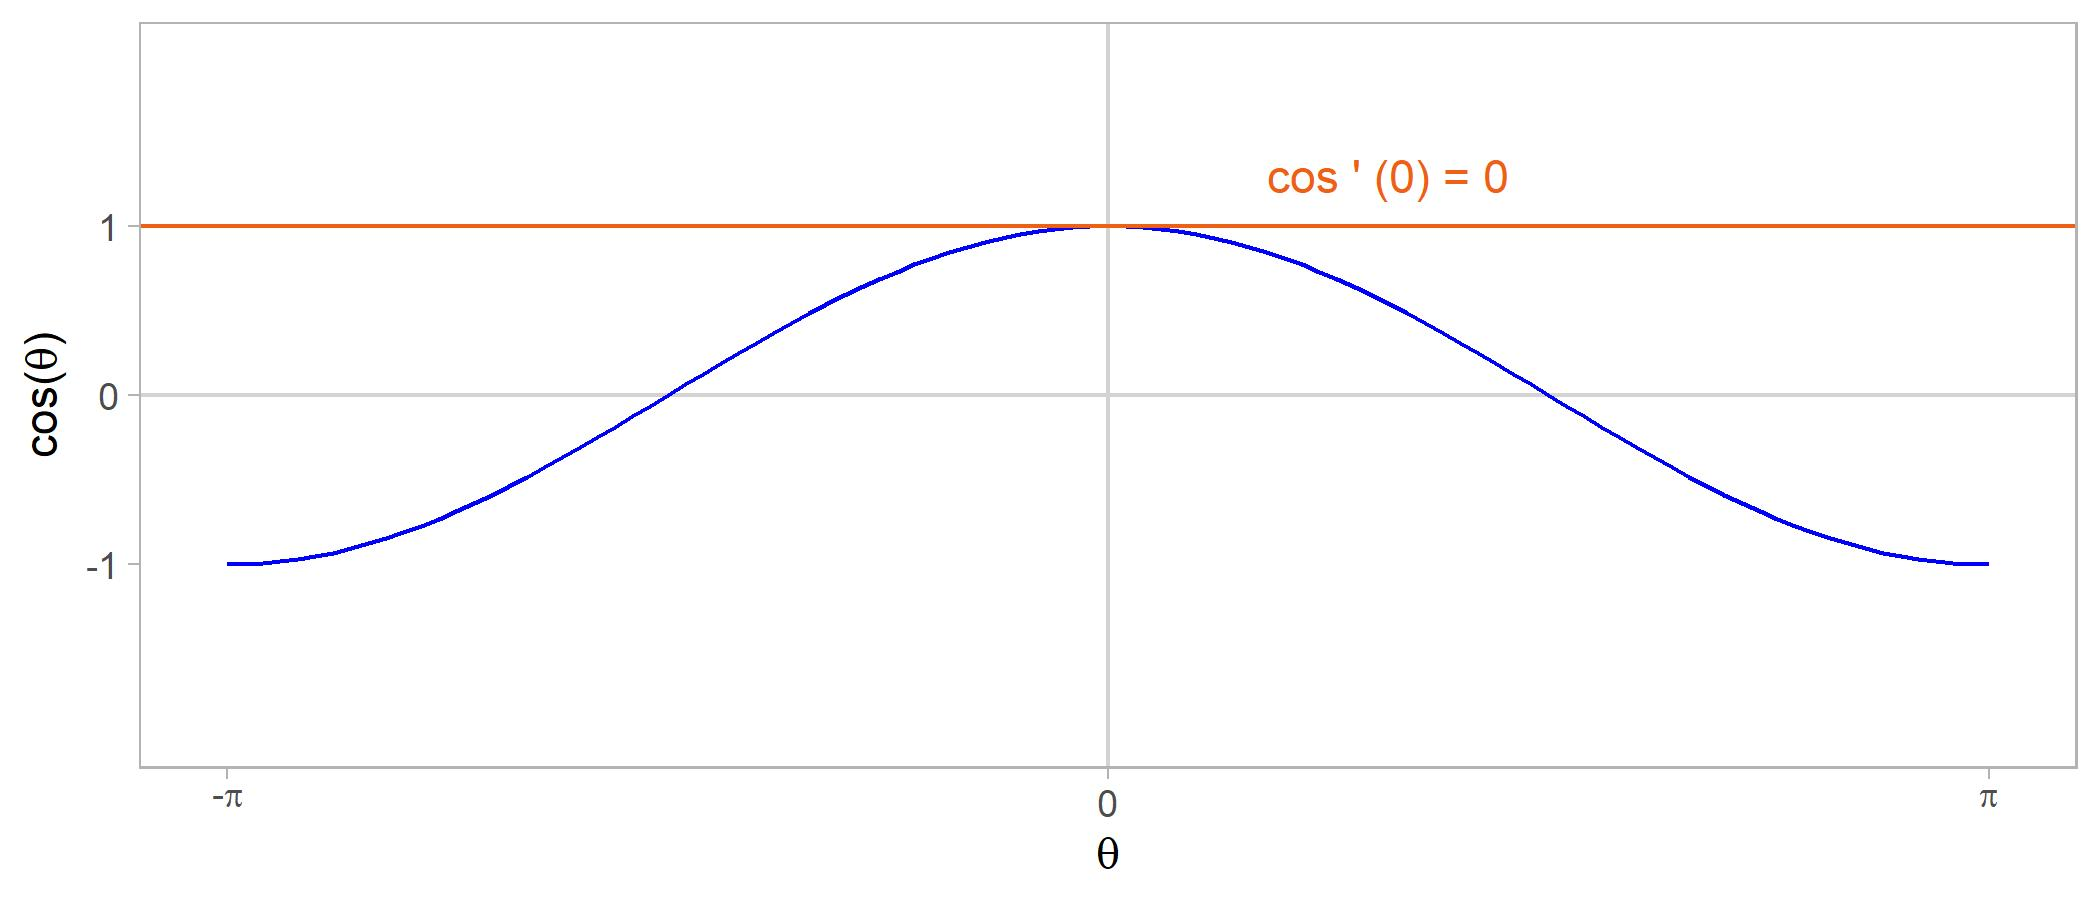
\includegraphics[scale=0.7]{img/deriv_cos_theta.jpg}
\end{figure}

Como vemos, justamente la pendiente de la recta tangente del $cos(\Theta)$ en $x = 0$, es cero. Es decir, no tiene pendiente.

Ahora recapitulemos para recordar por qué hemos realizado estas demostraciones. En un inicio, para el caso de la derivada del seno, llegamos hasta la siguiente expresión (pág. 52):
\[\frac{d}{dx}sen(x) = sen(x) \cdot \left(\lim_{\Delta \, x \to 0} \frac{cos(\Delta \, x) - 1}{\Delta \, x}\right) + cos(x) \cdot \left(\lim_{\Delta \, x \to 0} \frac{sen(\Delta \, x)}{\Delta \, x}\right)\]
Que, como vimos, es lo mismo que:
\[\frac{d}{dx}sen(x) = sen(x) \cdot cos'(x) + cos(x) \cdot sen'(x)\]
Cuando $x = 0$, con la información que manejamos podemos obtener lo siguiente:
\[\diff*{sen(x)}x[x=0] = sen(x) \cdot cos'(0) + cos(x) \cdot sen'(0)\]
\[\diff*{sen(x)}x[x=0] = sen(x) \cdot 0 + cos(x) \cdot 1\]
\[\diff*{sen(x)}x[x=0] = cos(x)\]
Del mismo modo lo podemos hacer con la derivada del $cos(x)$ en $x = 0$. Primero vamos a la aproximación de su línea tangente.
\[\diff*{cos(x)}x = \lim_{\Delta \, x \to 0} \frac{cos(x + \Delta \, x) - cos(x)}{\Delta \, x}\]
Al igual que con el $sen(x)$, en el numerador de este límite podemos usar la \textbf{fórmula de adición para el coseno}\footnote{$cos(a + b) = cos(a) \cdot cos(b) - sen(a) \cdot sen(b)$} en la expresión $cos(x + \Delta \, x)$.
\[\diff*{cos(x)}x = \lim_{\Delta \, x \to 0} \frac{[cos(x) \cdot cos(\Delta \, x) - sen(x) \cdot sen(\Delta \, x)] - cos(x)}{\Delta \, x}\]
El numerador también lo podemos agrupar por un denominador común, que en este caso es el $cos(x)$.
\[\diff*{cos(x)}x = \lim_{\Delta \, x \to 0} \frac{cos(x) \cdot cos(\Delta \, x) - cos(x) - [sen(x) \cdot sen(\Delta \, x)]}{\Delta \, x}\]
\[\diff*{cos(x)}x = \lim_{\Delta \, x \to 0} \frac{cos(x)(cos(\Delta \, x) - 1) - [sen(x) \cdot sen(\Delta \, x)]}{\Delta \, x}\]
\[\diff*{cos(x)}x = \lim_{\Delta \, x \to 0} \frac{cos(x)(cos(\Delta \, x) - 1)}{\Delta \, x} - \frac{sen(x) \cdot sen(\Delta \, x)}{\Delta \, x}\]
\[\diff*{cos(x)}x = \lim_{\Delta \, x \to 0} \left[cos(x) \left(\frac{cos(\Delta \, x) - 1}{\Delta \, x}\right) - sen(x)\left(\frac{sen(\Delta \, x)}{\Delta \, x}\right)\right]\]
\[\diff*{cos(x)}x = cos(x) \left(\lim_{\Delta \, x \to 0} \frac{cos(\Delta \, x) - 1}{\Delta \, x}\right) - sen(x)\left(\lim_{\Delta \, x \to 0} \frac{sen(\Delta \, x)}{\Delta \, x}\right)\]
Lo cual es lo mismo que:
\[\diff*{cos(x)}x = cos(x) \cdot cos'(x) - sen(x) \cdot sen'(x)\]
Y, si $x = 0$ en la derivada, entonces:
\[\diff*{cos(x)}x[x = 0] = cos(x) \cdot cos'(0) - sen(x) \cdot sen'(0)\]
\[\diff*{cos(x)}x[x = 0] = cos(x) \cdot 0 - sen(x) \cdot 1\]
\[\diff*{cos(x)}x[x = 0] = -sen(x)\]
En síntesis, podemos concluir que las derivadas del $sen(x)$ y del $cos(x)$, son:

\begin{enumerate}
\item[(a)] $\frac{d}{dx} sen(x) = cos(x)$
\item[(b)] $\frac{d}{dx} cos(x) = -sen(x)$
\end{enumerate}

Lo cual nos muestra una interesante relación que existe entre una derivada (de la función seno) con la otra (de la función coseno).

Por otra parte, si queremos saber en qué valor de $x$ o en cuál intervalo de $x$, la función $sen(x)$ o $cos(x)$ es cóncava hacia arriba o hacia abajo, podemos calcular las segundas derivadas de ambas funciones. Veamos la del $sen(x)$:
\[\frac{d^{2}}{dx^{2}} sen(x) = \frac{d}{dx} cos(x)\]
\[\frac{d^{2}}{dx^{2}} sen(x) = -sen(x)\]
Mientras que en el caso del $cos(x)$:
\[\frac{d^{2}}{dx^{2}} cos(x) = \frac{d}{dx} (-sen(x))\]
\[\frac{d^{2}}{dx^{2}} cos(x) = -cos(x)\]






























\end{document}